\documentclass[nochap,palatino]{apuntes}

\usepackage{fancysprefs}
\usepackage{natbib}
\usepackage{tikztools}
\usepackage{esint}
\usepackage{booktabs}

\bibliographystyle{plainnat}

\title{Variable Real}
\author{Guillermo Julián Moreno}
\date{15/16 C1}

\begin{document}
\pagestyle{plain}
\maketitle

\tableofcontents
\newpage
% Contenido.
\section*{Introducción y contenidos}

Estos son los apuntes tomados a lo largo del curso de Variable Real (5º curso Doble Grado) en la Facultad de Ciencias de la UAM, con el profesor Matteo Bonforte. La \fref{sec:TeoriaBasicaIntegral} se dedica a un repaso de los conceptos básicos de cursos anteriores de teoría de la integral y la medida (en \citep{ApuntesTIM} están los apuntes completos de esta asignatura). Estos conceptos se amplían con otros más avanzados en la \fref{sec:ComplementosTIM}.

En el apéndice \ref{chap:Discusiones} comentamos algunas discusiones interesantes relacionadas con la asignatura pero que no entran en el temario. Por último, el apéndice \ref{chap:Ejercicios} contiene algunos ejercicios y sus soluciones, sacados de los colgados en \url{http://uam.es/personal_pas/mbonfort/teaching.html}.

\section{Teoría básica de la integral y la medida}
\label{sec:TeoriaBasicaIntegral}

La teoría moderna de la integración sigue lo que se dice los tres principios de J.E. Littlewood (1885 - 1977), que dan de cierta forma la idea detrás de la integración según Lebesgue.

\begin{enumerate}
\item Cada conjunto (medible) es \textit{casi} una suma finita de intervalos.
\item Cada función absolutamente integrable es \textit{casi} continua.
\item Cada sucesión convergente puntualmente de funciones absolutamente integrable es \textit{casi} uniformemente convergente.
\end{enumerate}

Por ejemplo, uno de los problemas que se pretende resolver con la integral de Lebesgue es el de la convergencia de funciones. Con la integral de Riemann, para que se pueda intercambiar el límite con la integral (esto es, que $\int \lim f_n = \lim \int f_n$), la hipótesis necesaria es que $f_n$ converja uniformemente. La integral de Lebesgue si nos permitirá dar una noción más completa de convergencia (tercer principio) que nos permita intercambiar fácilmente la integral con el límite.

La teoría de Lebesgue también nos permite saltarnos problemas como el planteado por la \concept[Función\IS de Dirichlet]{función\IS de Dirichlet}, dada por \( \mathbb{D}(x) = \begin{cases} 1 & x ∈ ℚ \\ 0 & x ∈ ℝ \setminus ℚ \end{cases} \label{eq:Dirichlet} \)

$\mathbb{D}$ no es continua y por lo tanto no es integrable Riemann. La cuestión es que es \textit{casi} continua (segundo principio), así que con Lebesgue podemos quitarnos los problemas que aparecen en los puntos $x ∈ ℚ$ e integrarla sin problemas. Si uno tiene interés, en la \fref{sec:MotivacionLebesgue} explicamos por qué querría uno integrar monstruos como la función de Dirichlet.

En resumen, en todos los casos lo que tendremos es que, para todo ε, existe un conjunto de puntos de medida ε (los ``puntos malos'') de tal forma que nos lo podemos quitar y tendremos una función convergente, continua o integrable.

Este curso consistirá en la búsqueda y manejo de esos ``puntos malos'': veremos si podremos integrar en ellos, derivarlos y qué ocurre con las funciones en esos puntos.

Para trabajar con estas ideas desarrollaremos el concepto de las medidas que, por así decirlo, serán ``funciones generalizadas''. Por ejemplo, la \concept[Delta\IS de Dirac]{delta\IS de Dirac}, una ``función'' que vale cero en todo punto menos en $x = 0$, donde tiene un valor no concreto, se define en realidad como una medida dada por \[ δ_0 (A) = \begin{cases} 1 & 0 ∈ A \\ 0 & 0 ∉ A \end{cases} \] de tal forma que $\int_{ℝ} f(x) \dif δ = f(0)$.

\subsection{Conjuntos, espacios y funciones medibles}

A lo largo del curso trabajaremos con varias convenciones. Trabajaremos sobre la tres-tupla $(X, \mathcal{X}, μ)$, lo que llamaremos un espacio de medida. $X$ será el conjunto sobre el que mediremos. Normalmente será un subconjunto de $ℝ^n$, pero para el caso nos da igual. $\mathcal{X}$ será la σ-álgebra, el conjunto de subconjuntos medibles de $X$\footnote{Ver apuntes de TIM de Pedro.}. Por último, μ será la medida que usemos para integrar, usando la integral de Lebesgue.

¿Cuál es la diferencia entre las integrales de Riemann y de Lebesgue? Lo que se suele decir es que el primero mide en vertical y el segundo en horizontal. Una analogía es verlo como contar billetes. Por ejemplo, tenemos un billete de 50, uno de 20, dos de 10 y dos de 5. Riemann los contaría según le salen de la cartera, mientras que Lebesgue los agruparía primero en conjuntos de billetes iguales y luego contaría.

Mirando funciones, lo que hace Riemann es montar rectángulos en el eje $X$, mientras que Lebesgue los monta en el eje $Y$. De esta forma, la integral de Lebesgue es más estable, mientras que la de Riemann ve mejor las oscilaciones, por así decirlo. Un ejemplo curioso es el de la siguiente integral, \( \int_0^∞ \frac{\sin x}{x} \dif x \label{eq:IntRiemmanNoLeb} \) que es Riemann integrable pero no Lebesgue porque el valor absoluto no es integrable.

Para seguir trabajando con las medidas y poder integrar, necesitaremos saber qué funciones podemos medir y cuáles no.

\begin{defn}[Función\IS medible] Dados dos espacios de medida $(X, \mathcal{X}, μ),\,(Y, \mathcal{Y},ν)$, se dice que una función \stdf es medible si y sólo si $\inv{f}(E) ∈ \mathcal{X}\quad ∀E ∈ \mathcal{Y}$.
\end{defn}

También necesitaremos saber en qué σ-álgebra estamos trabajando. Nosotros usaremos normalmente la σ-álgebra de Borel:

\begin{defn}[{σ}-álgebra\IS de Borel] Denotada por \borel, es la σ-álgebra más que pequeña tal que los abiertos son medibles.\end{defn}

Otra $\salgb$ importante es la \concept{{σ}-álgebra\IS de Lebesgue}, denotada por $\lebg (ℝ^n)$. La relación entre esta y la de Borel es que la de Borel está contenida en la de Lebesgue: $\borel \subsetneq \lebg $. De hecho, $\lebg  \setminus \borel = \mathcal{N}$, que es el conjunto de conjuntos de medida Lebesgue 0. Por ejemplo, las uniones numerables tienen medida cero, como los racionales. Este es el gran avance de Lebesgue: identificar los conjuntos de medida 0 para poder integrar más funciones.

Algo que nos interesará es ver la composición de funciones.

\begin{prop}

\begin{enumerate}
\item La composición de funciones \borel-medibles es \borel-medible.
\item La composición de funciones \lebg-medibles no es, en general, \lebg-medible.
\item La composición de funciones \lebg-medibles con una de ellas continua sí es \lebg-medible.
\end{enumerate}
\end{prop}

\subsection{Medidas positivas}

\begin{defn}[Medida\IS positiva]\footnote{Positivas implicará a partir de ahora mayor \textit{o igual} que cero.} Una medida positiva (no negativa) en un espacio medible \meds es una función
\begin{align*}
\appl{μ}{\mathcal{X}&}{[0,+∞)} \\
E &\longmapsto μ(E) ≥ 0
\end{align*} y tal que
\begin{enumerate}
\item $μ(∅) = 0$.
\item $μ\left(\bigcup_{n=1}^∞ E_n\right) = \sum_{n=1}^∞ μ(E_n)$ con $E_n$ disjuntos dos a dos.
\end{enumerate}
\end{defn}

Hay dos nombres cocretos que nos interesarán. Si $μ(X) < ∞$, entonces se dice que μ es una \concept[Medida\IS finita]{medida\IS finita}. Si $μ(X) = 1$, será una \concept[Medida\IS infinita]{medida\IS de probabilidad}.

Un ejemplo de una medida que no es una función es la delta de Dirac que habíamos visto antes, que de hecho es una medida de probabilidad.

\begin{prop}[Propiedades de la medida][Medida!propiedades de] \label{prop:PropiedadesMedida} Dado un espacio medible \meas:

\begin{enumerate}
\item \textbf{Monotonía}: Si $E⊂F$, entonces $μ(E) ≤ μ(F)$.
\item \textbf{Sub-aditividad}: $μ\left(\bigcup_{n=1}^∞ E_n\right) ≤ \sum_{n=1}^∞ μ(E_n)$ (sólo es igual si los conjuntos son disjuntos).
\item \textbf{Convergencia monótona}: Dada una sucesión de conjuntos $E_1 ⊂ E_2 ⊂ \dotsb$, entonces $μ\left(\bigcup_{n=1}^∞ E_n\right) = \lim μ(E_n)$.
\item \textbf{Convergencia dominada}: Dada una sucesión decreciente de conjuntos $E_1 ⊃ E_2 ⊃ \dotsb$, entonces $μ\left(\bigcap E_n\right) = \lim μ(E_n)$.
\end{enumerate}
\end{prop}

\subsection{Teorema de Littlewood}

Al principio de esta sección veíamos los principios de Littlewood. Estos se traducen en teoremas para los que ya tenemos suficiente teoría para enunciarlos. El primer teorema, obviamente, corresponde al primer principio de Littlewood.

\begin{theorem} Para todo $ε>0$ y para todo $E∈\mathcal{X}$ con $μ(E) < ∞$, existe un $F∈\algbA⊂ \mathcal{X}$ tal que \[ μ\left((E\setminus F) ∪ (F \setminus E)\right) < ε \], con $\algbA$ la familia de conjuntos simples (intervalos, cuadrados o cubos según la dimensión, que son los que sabemos medir).
\end{theorem}

Lo que este teorema nos dice es que cualquier conjunto medible se puede aproximar tan bien como queramos por conjuntos simples, que es la idea del primer principio de Littlewood.

\subsection{Integración}

Dado \meas un espacio de medida, definiremos la integral de la siguientes formas. Primero iremos a lo más simple, que son (atención al nombre) las funciones simples:

\begin{defn}[Función\IS simple] Se dice que $\appl{f}{X}{[0, +∞)}$ es simple si $f$ es de la forma \[ f(x) = \sum a_i \ind_{E_i}(x) \] para $\set{E_i} ⊆ \mathcal{X}$.\end{defn}

Para funciones simples $\appl{f}{X}{[0,+∞)}$ como \[ \int_X f\ \dif μ = \sum_{i=1}^n a_i μ\set{\inv{f}(a_i)} \] Como notación, hay que tener en cuenta que \[ \set{\inv{f}(a_i)} \equiv \set{x∈X\tq f(x)=a_i} \]

Para funciones más complicadas usaremos, como siempre, límites. Dada $\appl{f}{X}{[0, +∞)}$ medible, definiremos su integral como \( \int_X f \dif μ = \sup_{\substack{0≤g≤f \\ g \text{ simple}}} \int_X g \dif μ \label{eq:ApproxIntegralFuncSimples} \)

Una observación que necesitaremos para poder usar esa definición es la siguiente proposición:

\begin{prop}\footnote{Demostrada en el \fref{ej:H1:SupremosMedibles}.} \label{prop:SupremoInfimoMedibles} Dada una familia de funciones $\appl{f_n}{X}{(-∞,+∞)}$ medibles, entonces $\sup f_n$ y $\inf f_n$ son medibles.\end{prop}

Con esto, ya podemos dar la definición de función integrable, que es bastante sencilla:

\begin{defn}[Función\IS integrable] Se dice que $f$ es integrable si y sólo si $\int f \dif μ < ∞$.\end{defn}

Ahora sólo nos falta aprender a integrar funciones negativas. Para eso definiremos las dos partes de una función: \(\begin{aligned}
f_+ &= \max\set{f,0} \\
f_- &= \max\set{-f, 0}\end{aligned} \label{eq:DescompFunc} \), de tal forma que $f = f_+ - f_-$, $\abs{f}= f_+ + f_-$ y entonces su integral es \[ \int_X f \dif μ = \int_X f_+ \dif μ - \int_X f_- \dif μ \]

Análogamente podemos hacer la integral de funciones complejas descomponiendo \[ f = (\Re f)_+ - (\Re f)_- + \imath (\Im f)_+ - \imath (\Im f)_- \] e integrando igual que antes.

Vamos a ver ahora las propiedades de las integrales.

\begin{prop} Dada $\appl{f}{X}{[-∞,+∞]}$, entonces

\begin{enumerate}
\item $f$ es integrable si y sólo si $\abs{f}$ es integrable\footnote{Esto en Riemann no es cierto, ver el contraejemplo de la \fref{eq:IntRiemmanNoLeb}.}, esto es, que $\int_X \abs{f} \dif μ < ∞$. En este caso decimos $f ∈ \lebg^1\meas \equiv \lebg^1 (X) \equiv \lebg_μ^1 (X) \equiv \lebg^1$, según lo que demos por supuesto en cada caso, donde $\lebg^1$ es el espacio vectorial de las funciones absolutamente integrables.
\item La aplicación que lleva cada función a su integral $f\longmapsto \int_X f \dif μ$ es lineal. Es fácil ver que $αf + βg = α \int_X f \dif μ + β \int_X g\dif μ$.
\item \concept{Desigualdad\IS triangular en $\lebg^1$}. Dada $\appl{f}{X}{ℂ}$ absolutamente integrable, entonces $\abs{\int f \dif μ} ≤ \int \abs{f}\dif μ$.
\item \textbf{Comparación}. Si $0 ≤ f ≤ g$, entonces $0 ≤ \int f \dif μ ≤ \int g \dif μ$. Además, si $f ≥ 0$ entonces $\int f = 0$ si y sólo si $f = 0$ en casi todo punto\footnote{$f = 0$ en casi todo punto si $∃N ⊂ X$ tal que $μ(N) = 0$ con $f ≠ 0$ en $N$.}. En el otro sentido, si $\int\abs{f} = 0$ entonces $f \equiv 0$ en casi todo punto.
\item Una función integrable se puede modificar todo lo que se quiera en un conjunto de medida nula mantieniendo su integral constante. Esta propiedad será un problema para definir los espacios de funciones integrables, como veremos más tarde.
\item $f ∈ \lebg^1_μ(X;ℂ)$ entonces $f$ es finita en casi todo punto.
\item La integral de Lebesgue ``generaliza'' la de Riemman, en el sentido de que todas las fórmulas como integración por partes, jacobianos y cambios de coordenadas son las mismas.
\end{enumerate}
\end{prop}

\begin{proof}
\begin{enumerate}
\item Si $f$ es integrable, entonces podemos descomponerla en $f_+$ y $f_-$, definidas como en \eqref{eq:DescompFunc} e integrables por construcción. En ese caso, $\abs{f} = f_+ + f_-$ es suma de funciones integrables y será también integrable.

Por otra parte, si $\abs{f}$ es integrable, entonces para cualquier posible descomposición $\abs{f} = f_+ + f_-$ tendremos que \[ \int_X f \dif μ = \int_X f_+ \dif μ - \int_X f_- \dif μ \eqreasonup[≤]{$f_- ≥ 0$} \int_X f_+ ≤ \int_X \abs{f} \dif μ < ∞ \]

\item Trivial.

\item Operamos y vemos que \[ \abs{\int f \dif μ} = \abs{\int f_+ \dif μ - \int f_- \dif μ} ≤ \int f_+ \dif μ + \int f_- \dif μ = \int\abs{f} \dif μ\]

\item Bastante trivial también.

\item Igualmente trivial. Medida cero implica que la integral valdrá cero y esa modificación no afectará en nada al valor final.

\item Si hubiese un conjunto de medida no nula en el que la función no es finita, la integral del valor absoluto no daría un valor finito y por lo tanto no sería integrable.
\end{enumerate}
\end{proof}

La primera propiedad de la proposición merece un repaso adicional. En general, no sólo querremos ver si $\abs{f}$ es integrable, también buscaremos ver si lo son sus potencias.

\begin{defn}[Función\IS absolutamente integrable de orden $p$] Decimos que $f$ es absolutamente integrable de orden $p$ con $p > 0$ si y sólo si $\abs{f}^p$ es absolutamente integrable, esto es, que \[ 0 ≤ \int_X \abs{f}^p \dif μ < ∞ \]. Por notación, diremos que $f ∈ \lebg^p\meas$
\end{defn}

Como comentábamos en la proposición, es interesante ver que los espacios $\lebg^p$ son espacios vectoriales. Si tomamos $α,β ∈ ℂ$ y $f,g ∈ \lebg^p$, entonces querremos ver si $αf + βg ∈ \lebg^p$. Operando, podemos descomponer \[ \int\abs{αf+βg}^p \dif μ ≤ C_p \int \left(\abs{αf}^p + \abs{βg}^p\right) ≤ C_p \left(\abs{α}^p \int \abs{f}^p + \abs{β}^p \int \abs{g}^p \right) < ∞ \] y ver que efectivamente la combinación lineal también es absolutamente integrable.

\subsubsection{Teoremas de integración}

Ahora vamos con varios teoremas sobre integración.

\begin{theorem}[Teorema\IS de Fubini-Tonelli] Dada $\appl{f}{X×Y}{ℂ}$ medible, entonces \[ \iint\limits_{X×Y} f \dif μ \dif ν = \int_X \underbrace{\left(\int_Y f(x,y) \dif ν(y)\right)}_{F_1(x)} \dif μ(x) = \int_Y \underbrace{\left(\int_X f(x,y) \dif μ(x)\right)}_{F_2(y)} \dif ν(y) \] con $F_1$, $F_2$ medibles.

Concretamente, Tonelli nos da la medibilidad para funciones no negativas y Fubini la condición de integrabilidad.

\label{thm:FubiniTonelli}
\end{theorem}

Este teorema nos dice cómo integrar en varias coordenadas y además nos da una introducción a lo que deberían de ser las medidas producto. En la primera parte de la ecuación, estamos midiendo el conjunto $X × Y$ con respecto a la medida $μ×ν$, y en las otras dos integrales estamos traduciendo eso al producto de dos medidas. Definamos esto más concretamente.

\begin{defn}[Medida\IS producto] \label{def:MedidaProducto} Dados dos espacios medibles $\meds[X], \meds[Y]$ con medidas μ y ν respectivamente, consideramos $\algb{X} \otimes \algb{Y}$ la σ-álgebra producto en el espacio producto $X × Y$ generada por conjuntos $B_1 × B_2$ con $B_1 ∈ \algb{X}$ y $B_2 ∈ \algb{Y}$.

Entonces, definimos la medida producto $μ×ν$ como la medida en el espacio $(X×Y, \algb{X} \otimes \algb{Y})$ dada por \[ (μ×ν)(B_1×B_2) = μ(B_1) · ν(B_2)\] con $B_1 ∈ \algb{X}$ y $B_2 ∈ \algb{Y}$.
\end{defn}

Esta definición nos permitirá trabajar bien con integrales múltiples, adaptando las medidas a esas condiciones.

\seprule

Otro teorema, que se corresponde con el tercer principio de Littlewood.

\begin{theorem}[Teorema\IS de Egorov] Dada $\appl{f}{X}{ℂ}$ medible y $f_n \convs f$ en casi todo punto en $A⊆X$, entonces $f_n \convs f$ casi uniformemente en $A$. Esto es, converge uniformemente salvo en un conjunto de medida cero. Más formalmente, $∀ε>0$ existe un $N_ε⊆A$ tal que $f_n \convs f$ en $A\setminus N_ε$ y $0 ≤ μ(N_ε) < ε$.
\end{theorem}

La prueba de este teorema es sencilla y bonita:

\begin{proof} Para $k,n ∈ ℕ$ definimos \[ E_n(k) = \sum_{m=n}^∞ \set{x∈X \tq \abs{f_m(x) - f(x)} > \frac{1}{k}} \] como el conjunto de puntos en los que la función se aleja del límite. Para todo $k$ fijo, es fácil ver que $E_n(k) ⊇ E_{n+1}(k) ⊇ \dotsb $ y además \[ μ\left(\bigcap_{n=1}^∞ E_n(k)\right) = 0 \] (si no fuese así, tendríamos un conjunto de puntos de medida no nula en la que la sucesión no converge, y hemos dicho que convergía en casi todo punto).

Por convergencia dominada de las medidas (ver \fref{prop:PropiedadesMedida}), sabemos que $\lim_{n\to \infty} μ(E_n(k)) = μ\left(\bigcap E_n\right) = 0$.

Ahora la prueba se acaba de forma bastante sencilla: dado $ε > 0$ y $k∈ℕ$, siempre podremos encontrar un $m_k$ tal que $μ(E_{m_k}(k)) ≤ \frac{ε}{2^k}$. Entonces, definimos $E = \bigcup_{k=1}^∞ E_{m_k}(k)$, que será el conjunto donde la sucesión no se aproxima uniformemente a $f$. Por definición, \[ μ(E) ≤ \sum_{n≥1} μ(E_{n_k}) = \sum_{k≥1} \frac{ε}{2^k} ≤ ε \], esto es, podemos hacer la medida de ese conjunto tan pequeña como queramos, así que tendremos convergencia uniforme salvo en un conjunto de medida cero.
\end{proof}

\begin{theorem}[Teorema\IS de Lusin] \label{thm:Lusin} Dada $\appl{f}{X}{ℂ}$ medible con $μ(X) < ∞$, entonces $f$ es casi continua, que como viene siendo hasta ahora significa que $f$ es continua salvo en un conjunto de medida cero. Esto es, que $∀ε>0$ existe un $N_ε⊆X$ tal que $f$ es continua en $X\setminus N_ε$ y $μ(N_ε) < ε$.
\end{theorem}

\subsubsection{Integración en coordenadas polares}

Además de las coordenadas lineales, en los reales podemos usar (y lo haremos habitualmente) las coordenadas polares o esféricas, esto es, coordenadas basadas en el uso de una esfera o equivalente en $ℝ^n$ en lugar del cuadrado/cubo/cosa.

En $ℝ^2$, las coordenadas polares nos dan una integral $\dif x \dif y = r \dif r \dif θ$, y en $ℝ^3$ tenemos $\dif x \dif y \dif x = r^2 \sin φ \dif r \dif θ \dif φ$. Esto nos da una intuición que nos dice que la medida en coordenadas esféricas en $ℝ^n$ está relacionada con la medida del radio $r^{n-1}$ y con un ``algo'' que parece estar relacionado con la medida de la superficie de la esfera unidad.

Podríamos tratar de generalizar ese ``algo'' haciendo integrales en más dimensiones, pero hay otra forma más fácil sin necesidad de usar cosenos y senos por todas partes.

Como viene siendo habitual, primero haremos nuestras definiciones formales.

\begin{defn}[Coordenadas\IS polares] Sea $\set{x ∈ ℝ^n \tq \md{x} = 1} = \bbs^{n-1}$ la esfera unidad en $ℝ^n$. Entonces, si $x ∈ ℝ^n \minuszero$ las coordenadas polares de $x$ son
\begin{align*}
r  &= \md{x} ∈ (0,∞) \\
θ &= \frac{x}{\md{x}} ∈ \bbs^{n-1} \\
\end{align*}
con el cambio de coordenadas dado por la aplicación biyectiva
\begin{align*}
\appl{Φ}{ℝ^n\minuszero&}{(0,∞)×\bbs^{n-1}} \\
x &\longmapsto (r,θ)
\end{align*} con inversa continua $\inv{Φ}(r,θ) = rθ$.
\end{defn}

Dadas estas coordenadas, necesitamos definir una medida. Lo fácil será hacerlo usando $ℝ^n$, que para eso sabemos medirlo perfectamente. Dado que $Φ$ es continua con inversa continua, nos lleva de conjuntos de Borel a conjuntos de Borel\footnote{Ver \href{http://mathoverflow.net/questions/63677/polar-coordinates-and-borel-sets}{MathOverflow} para una explicación algo más detallada de esto, aunque tampoco mucho más.}. Así, podemos definir $μ_\ast$ como la medida de Borel en $(0,∞)×\bbs^{n-1}$ inducida por Φ desde la medida $μ$ de Lebesgue en $ℝ^n$. En otras palabras, \[ μ_\ast (E) = μ(\inv{Φ}(E)) \]

De momento no hemos hecho nada más que decir algo obvio: que la medida de un conjunto $E$ de coordenadas esféricas debería ser la misma que la medida de ese conjunto de puntos tomados como coordenadas cartesianas. Esto nos da una vía para construir $μ_\ast$.

\begin{theorem} \citep[Teorema 2.49]{folland99} Sea $ρ=ρ_n$ la medida en $(0,∞)$ dada por $ρ(E) = \int_E r^{n-1}\dif r$. Entonces existe una única medida de Borel $σ = σ_{n-1}$ en $\bbs^{n-1}$ tal que $μ_\ast = ρ × σ$. Si $f$ es Borel-medible en $ℝ^n$ y $f ≥ 0$ o $f ∈ \lebg^1(μ)$, entonces
\(
\int_{ℝ^n} f(x) \dif x = \int\limits_0^{∞} \int\limits_{\bbs^{n-1}} f(rθ) r^{n-1} \dif σ(θ) \dif r
\label{eq:MedidaPolares} \)
\end{theorem}

\begin{proof} Es fácil ver que, si $f$ es la función característica de un conjunto (esto es, $f \equiv \ind_E$), entonces \eqref{eq:MedidaPolares} es simplemente otra forma de decir que $μ_\ast = ρ × σ$ (ver definición de \nlref{def:MedidaProducto}).

En ese caso, se puede generalizar a funciones genéricas igual que hacíamos en \eqref{eq:ApproxIntegralFuncSimples}, usando aproximación por funciones simples. Así, sólo tenemos que construir σ para que esa definición de integral, que coincide con lo que decíamos al principio de la sección: que la medida en coordenadas esféricas está relacionada con el radio $r^{n-1}$ y un ``algo'' relacionado con la medida de la esfera unidad (la superficie), que será $\difσ(θ)$.

Si $E$ es un conjunto de Borel en $\bbs^{n-1}$ y $a > 0$, sea \[ E_a = \inv{Φ}\left((0,a] × E\right) = \set{rθ \tq 0 < r ≤ a, θ ∈ E } \], en otras palabras, el conjunto de todos los puntos con ángulos contenidos en $E$ y radios desde $0$ hasta $a$.

Dado que \eqref{eq:MedidaPolares} se tiene que cumplir cuando en particular $f = \ind_{E_1}$, nuestra medida $σ$ deberá cumplir la relación \( μ(E_1) = \int_0^1\int_E r^{n-1} \dif σ(θ) \dif r = σ(E) \int_0^1 r^{n-1} \dif r = \frac{σ(E)}{n} \label{eq:PrIntPolares:MedMuSigma}  \)

Consecuentemente, definimos σ para que sea $σ(E) = n · μ(E_1)$. Dado que la aplicación $E\mapsto E_1$ lleva conjuntos de Borel a conjuntos de Borel y conmuta con la unión, intersección y complemento, entonces esta σ que hemos definido es una medida de Borel en $\bbs^{n-1}$: vamos por el buen camino.

Además, dado que $E_a$ es la imagen de $E_1$ por la aplicación $x \mapsto ax$, se sigue de \citep[Teorema 2.44]{folland99} que \[ μ(E_a) = a^n μ(E_1) \], lo que nos reduce el problema a saber medir $E_1$, ya que la parte del radio se resuelve muy fácilmente: si tomamos $0 < a < b$ y consideramos el conjunto $(a,b] × E$, cuya imagen inversa por $Φ$ es $E_b \setminus E_a$, entonces
\begin{multline}
μ_\ast\left((a,b] × E\right) = μ(E_b \setminus E_a) = μ(E_b) - μ(E_A) = \frac{b^n-a^n}{n}σ(E) = \\
= \left( \int_a^b r^{n-1}\dif r\right) σ(E) = ρ((a,b]) · σ(E) = (ρ × σ) \left((a,b]×E\right)
\label{eq:PrIntPolares:MedProducto}\end{multline}

Fijado un conjunto de Borel $E$ de $\bbs^{n-1}$, consideramos $\algbA_E$ la colección de uniones finitas y disjuntas de conjuntos de la forma $(a,b] × E$, que es un álgebra en $(0,∞)×E$ que genera la σ-álgebra $\mathcal{M}_E = \set{A×E \tq A ∈ \borel_{(0,∞)}}$. Por el cálculo de \eqref{eq:PrIntPolares:MedProducto} tenemos que $μ_\ast = ρ × σ$ en $\algbA_E$, y por ser la medida única \citep[Teorema 1.14]{folland99} entonces esta ecuación también se cumple en $\mathcal{M}_E$. Como $\bigcup \set{\mathcal{M}_e \tq E ∈ \borel_{\bbs^{n-1}}}$ no es más que los conjuntos de Borel en $(0,∞) × \bbs^{n-1}$, así que por el mismo teorema de unicidad tenemos que $μ_\ast = ρ × σ$ en todos los conjuntos de Borel.\footnote{No es culpa mía, Folland lo explica así de mal.}
\end{proof}

\begin{corol} Si $f$ es una función medible en $ℝ^n$ tal que $f(x) = g(\abs{x})$ para alguna función $g$ en $(0,∞)$, entonces \( f(x) \dif x = σ(\bbs^{n-1}) \int_0^{∞} g(r) r^{n-1}\dif r \label{eq:IntegralPolares} \)
\label{crl:MediblePolares1}
\end{corol}

\begin{prop} \citep[Proposición 2.53]{folland99} Si $a > 0$, entonces \( \int_{ℝ^n} e^{-a\md{x}^2} \dif x = \left(\frac{π}{a}\right)^\frac{n}{2} \label{eq:IntegralExp2} \)
\end{prop}

\begin{proof} Denotamos la integral por $I_n$. Para dimensión $n=2$ podemos calcular $σ(\bbs^1)$, que es $2π$, así que por el \fref{crl:MediblePolares1} tenemos que \[ I_2 = 2π\int_0^∞ re^{-ar^2} \dif r = \eval{- \left(\frac{π}{a}\right) e^{-ar^2}}_0^∞ = \frac{π}{a} \]

Dado que $e^{-a\md{x}^2} = \prod_{j=1}^n e^{-ax_j^2}$, por el teorema de Tonelli (\ref{thm:FubiniTonelli}) tenemos que $I_n=(I_1) ^ n$. En particular $I_1 = (I_2)^{\frac{1}{2}}$, y la proposición sigue naturalmente.
\end{proof}

Este resultado nos permitirá calcular $σ(\bbs^{n-1})$ para todo $n$ en términos de la función $Γ$.

\begin{prop} \citep[Proposición 2.54]{folland99} \label{prop:MedidaSn} \( \label{eq:MedidaSn} σ(\bbs^{n-1}) = \frac{2π^\frac{n}{2}}{Γ(n/2)} \)
\end{prop}

\begin{proof} Combinamos \eqref{eq:IntegralPolares} y \eqref{eq:IntegralExp2}, tomando $a = 1$ por simplificar \[ π^\frac{n}{2} = \int_{ℝ^n} e^{-\md{x}^2} \dif x = σ(\bbs^{n-1}) \int_0^{∞} r^{n-1} e^{-r^2} \dif r \]

Ahora, idea feliz, nos acordamos de la integral de la función Gamma (la que se puede considerar como la extensión del factorial a los reales): \[ Γ(n) = \int_0^∞ x^{n-1} e^{-x} \dif x \] así que podemos hacer la sutitución $s = r^2$ para seguir operando:

\[ π^\frac{n}{2} = σ(\bbs^{n-1}) \int_0^{∞} r^{n-1} e^{-r^2} \dif r = \frac{σ(\bbs^{n-1})}{2} \int_0^∞ s^{\frac{n}{2} - 1} e^{-s} \dif s = \frac{σ(\bbs^{n-1})}{2} Γ\left(\frac{n}{2}\right) \] y despejando ya nos quedaría \eqref{eq:MedidaSn}, lo que queríamos demostrar.
\end{proof}

Podemos usar esta proposición para sacar la medida de la esfera unitaria en $n$ dimensiones.

\begin{corol} \label{crl:MedidaBn} Sea $\bola_r^N = \set{x ∈ ℝ^N \tq \md{x} < r}$. Entonces \( μ(\bola_r^N) = r^N\frac{π^{n/2}}{Γ\left(\frac{n}{2} + 1\right)} = r^N ω_N \label{eq:MedidaBn} \)
\end{corol}

\begin{proof} Según \eqref{eq:PrIntPolares:MedMuSigma}, que nos relaciona la medida $σ(E)$ con la de $μ((0,1] × E)$, tenemos que $μ(\bola_1^N) = n^{-1} σ(\bbs^{N -1})$, así que \[ μ(\bola_1^{N}) =  \frac{2π^\frac{n}{2}}{nΓ(n/2)} = \frac{π^\frac{n}{2}}{\frac{1}{2}n Γ\left(\frac{n}{2}\right)} =\frac{π^\frac{n}{2}}{Γ\left(\frac{n}{2} + 1\right)}  \]

Para radios distintos de $1$, sólo tenemos que multiplicar por $r^N$.
\end{proof}

A modo de curiosidad, podemos ger que $ω_N \convs 0$, esto es, que la medida de la bola se va a cero según aumentan las dimensiones.

Para practicar la integración en polares, podemos ver algunas integrales. Por ejemplo, veamos \( \int_{ℝ^n}\frac{1}{\md{x}^α} \dif x \label{eq:IntPolaresModAlpha} \) para $α ∈ ℝ$. Si usamos el \fref{crl:MediblePolares1}, con $f(x) = g(\md{x})$ para $g(r) = \frac{1}{r}$ tenemos que \( \label{eq:IntPolaresModAlpha2} \int_{ℝ^n}\frac{1}{\md{x}^α} \dif x = \frac{2π^{n/2}}{Γ(n/2)} \int_0^∞ g(r) r^{n-1} \dif r = \frac{2π^{n/2}}{Γ(n/2)} \int_0^∞ r^{n-1 - α} \dif r\)

Comprobar que $\int_{ℝ^N} \frac{1}{(1 + \abs{x})^α} < ∞$ para cierto $α$ encontrarlo (pone algo de cambio a polares) y luego que $\int_{B_1(0)} \frac{1}{\abs{x}^{β}} < ∞$ y $\int_{B_1(0)} \frac{1}{(1-\abs{x})^α}$.

\subsection{Convergencia de funciones}

A lo largo del curso, nos interesará estudiar y entender la convergencia de funciones. Sin embargo, como hemos visto en otros cursos, hay varios tipos de convergencia y varios resultados sobre lo que les ocurre a las funciones y a la integral.

Antes de entrar en materia, una pequeña definición que no hemos visto, que es la del supremo esencial. Es análogo a todo lo que estamos haciendo hasta ahora, extendiendo conceptos no a todos los puntos sin a todos ``salvo un conjunto de medida cero''. En el caso del supremo es un poco más delicado, así que vamos a hacerlo bien.

\begin{defn}[Supremo\IS esencial] Sea $\appl{f}{X}{ℝ}$ una función y \meas nuestro espacio de medida habitual. Definimos entonces el supremo esencial como \[ \essup_{x∈X} f(x) = \inf \set{a ∈ ℝ \tq μ\left(\inv{f}((a, ∞))\right) = 0} \]

En otras palabras, es el mayor valor de $f$ tal que por encima sólo hay un conjunto de valores de medida cero.
\end{defn}

Por ejemplo, es fácil ver que $\sup_{x∈(0,1)} x^n = 1$; pero $\essup_{x∈(0,1)}x^n$ ya es más complicado. Lo podemos ver sin cosas esenciales: \[ x^n \convs l(x) = \begin{cases} 0 & x < 1 \\ 1 & x = 1 \end{cases} \], converge puntualmente en todo punto pero no uniformemente (el límite no es continuo). Además, es fácil ver así que $\essup_{x∈(0,1)} x^n = 0$, ya que la función sólo es mayor que ese valor en un conjunto de medida cero (un único punto).

Después de esta ligeramente útil introducción, vamos a ver los teoremas.

\subsubsection{Teoremas de convergencia de funciones}

\begin{theorem}[Teorema\IS de convergencia monótona] (o teorema de Beppo-Levi) \label{thm:ConvMonotona}
Dado un espacio de medida \meas y una sucesión monótona de funciones $0 ≤ f_1 ≤ \dotsb ≤ f_n ≤ \dotsb$ medibles, entonces  \[ \int_X \lim_n f_n \dif μ = \lim_n \int_X f_n \dif μ \]

Se puede extender a sucesiones decrecientes simplemente cambiado el signo.
\end{theorem}

Hay una variación sutil de este teorema: es prácticamente lo mismo pero aun así lo veremos.

\begin{theorem}[Teorema\IS de convergencia monótona para series] \label{thm:ConvMonotonaSeries} Dada una sucesión de funciones $\appl{f_n}{X}{[0,+∞]}$ medibles y no negativas, entonces \[ \int_X \sum_n f_n \dif μ = \sum_n \int f_n \dif μ\]
\end{theorem}

¿Por qué decimos que es casi lo mismo? Si definimos las sumas parciales $S_N = \sum_{n=1}^N f_n$ tendremos una sucesión monótona creciente y podremos aplicar el \fref{thm:ConvMonotona}. Ver el \fref{ej:H1:ConvMonotonaSeries} para la explicación más extensa.

\begin{theorem}[Lema\IS de Fatou] \label{thm:Fatou} Dada una sucesión de funciones $0 ≤ f_n$ no negativas y medibles, entonces \[ \int_X \liminf_n f_n \dif μ ≤ \liminf_n \int_X f_n \dif μ \]
\end{theorem}

Para saber el $\limsup$, vamos al siguiente lema:

\begin{theorem}[Lema\IS de Fatou-Lebesgue] \label{thm:FatouInverso} (también llamado de Fatou inverso) Dada una sucesión de funciones $f_n$ $0 ≤ f_n ≤ g$, con $g$ integrable, entonces \[ \limsup_n \int f_n \dif μ ≤ \int_X \limsup f_n \dif μ \]
\end{theorem}

Para probar este lema, simplemente hay que aplicar el lema de Fatou normal (\ref{thm:Fatou}) a $F_n = g - f_n ≥ 0$.

\begin{theorem}[Teorema\IS de convergencia dominada] \label{thm:ConvDominada} Dada una sucesión $f_n \convs f$ en casi todo punto, si existe una función $g$ integrable y no negativa tal que $\abs{f_n} ≤ g$ entonces \[ \int_X \lim_n f_n \dif μ = \lim_n \int f_n \dif μ\]
\end{theorem}

\begin{proof}[Esquema]
Para la prueba del teorema, simplemente usaríamos los dos teoremas \ref{thm:Fatou} y \ref{thm:FatouInverso}. Si existe el límite de las integrales, existen los límites superior e inferior y tenemos las desigualdades.
\end{proof}

\begin{theorem}[Teorema\IS de convergencia dominada para series] Dada una sucesión de funciones $f_n$ medibles tal que $f_n \convs f$ en casi todo punto. Entonces si $\sum_n \int \abs{f_n}\dif μ < ∞$, entonces  \[ \int_X \sum_n f_n \dif μ = \sum_n \int f_n \dif μ\]
\end{theorem}

Además de los teoremas, nos interesará ver varios ejemplos de series especiales que nos ``fastidien'' los teoremas.

Uno sencillo para Fatou es \( f_n(x) = \begin{cases} \frac{1}{n} & x ∈ [0,n] \\ 0 & x ∉ [0,n] \end{cases} \label{eq:ContrajemploFatou1} \), que convege puntualmente a 0 uniformemente. Sin embargo, $\int_ℝ f_n \dif x = 1$ para todo $n$. Entonces tenemos un menor estricto en la ecuación del lema de Fatou (\ref{thm:Fatou}).

Como ejercicio, podemos ver qué le ocurre a la función \[ f_n(x) = \begin{cases} \frac{-1}{n} & x ∈ [n, 2n] \\ 0 & x ∉ [n, 2n] \end{cases} \], que converge uniformemente a cero pero la integral es -1 para todo $n$. Podríamos tratar de usar el \nref{thm:ConvDominada}, pero es imposible encontrar una función $g$ que domine a $f_n$ y sea integrable: como el soporte de $f_n$ se mueve hacia infinito con $n$, la $g$ que domine deberá ser distinta de cero en un intervalo $(x_0, ∞)$ y eso no va a ser integrable.

\section{Complementos de teoría de la integral y la medida}
\label{sec:ComplementosTIM}

Hasta ahora, hemos hecho un repaso de los conceptos básicos del curso de teoría de la integral y la medida (véase \citep{ApuntesTIM} para los apuntes completos). Ahora lo que vamos a hacer será ampliar esos conocimientos con teoremas y definiciones extra que necesitaremos a lo largo de este curso de Variable Real.

Lo primero que haremos será ir con el primer ``teorema de verdad del curso'', que nos va a dar el término que falta en el \nref{thm:Fatou}. Este es un resultado que se ha obtenido en los años 80, bastante después de los resultados de Lebesgue y Fatou. Es además un teorema con muchas aplicaciones y con una prueba muy bonita.

\begin{theorem}\label{thm:LiebLoss}\citep[Teorema 1.9]{liebLoss01}, publicado en \cite{brezis1983relation}. Dado un espacio de medida \meas y una sucesión de funciones $\appl{f_n}{X}{ℂ}$ medibles, con $f_n \convs f$ en casi todo punto y $f$ medible\footnote{Esto viene gratis por ser $f_n$ medibles.}, y además\footnote{Pedimos una versión más general de la función dominante de otros teoremas: simplemente queremos todas las funciones de la familia sean similares en su integral (o algo así).} $\abs{f_n}^p$ es integrable y $\int \abs{f_n}^p ≤ C$ para todo $n$. Entonces \[ \lim_{n\to ∞ } \int_X\abs{\abs{f_n}^p - \abs{f}^p - \abs{f_n - f}^p} \dif μ = 0\]
\end{theorem}

¿Qué tiene que ver ese churro con el lema de Fatou? Si recordamos la desigualdad triangular ($\abs{\abs{a} - \abs{b}} ≤ \abs{a-b}$), tomando $a = \abs{f_n}^p - \abs{f}^p$ y $b = \abs{f_n -f}^p$, tendremos que \[ \lim_f \int \abs{\abs{f_n}^p - \abs{f}^p} - \lim \int \abs{f_n - f}^p ≤ \lim \int \abs{\abs{f_n}^p - \abs{f}^p - \abs{f_n - f}^p} \dif μ = 0\], por lo que quitando también los límites nos quedará \( \int \abs{\abs{f_n}^p - \abs{f}^p} = \int\abs{f_n -f}^p + o(n) \label{eq:LiebLossOn}\) con $o(n) \convs 0$.

Para ver qué ocurre exactamente, podemos tratar de aplicarlo a \eqref{eq:ContrajemploFatou1}, una sucesión de funciones para las que vimos que había un menor estricto en el \nlref{thm:Fatou}: \[ f_n(x) = \begin{cases} \frac{1}{n} & x ∈ [0,n] \\ 0 & x ∉ [0,n] \end{cases} \]

Podemos aplicar perfectamente el \fref{thm:LiebLoss}: $f_n$ es medible para todo $n$, la convergencia es a $f(x) = 0$ en casi todo punto y $\int\abs{f_n}^p ≤ 1$ para todo $n,p$. Sustituyendo ahora en \eqref{eq:LiebLossOn} tenemos que \[ \int \abs{f_n}^p = \int \abs{f_n}^p + o(n)\] con $o(n) = 0$ sin ninguna dificultad porque $f = 0$, así que creo que me he equivocado y en realidad había que usar otra sucesión.

En cualquier caso, en general en la fórmula de Fatou nos quedará un ``resto'' (igual que el $o$ de Taylor): \[ \liminf \int \abs{f_n}^p ≥ \int \liminf \abs{f_n}^p + \int \abs{f-f_n}^p + o(n) ≥ 0 \]

Antes de ir con la prueba del \fref{thm:LiebLoss}, vamos a ver dos desigualdades que necesitaremos usar.

\begin{prop}[Desigualdad\IS de Young] \label{prop:Young} Dados $p > 0$ y $a,b≥0$, entonces \[ (a+b)^p ≤ C_p (a^p + b^p)\] con $C_p$ una constante que puede depender de $p$.
\end{prop}

\begin{proof} Sin pérdida de generalidad, podemos simplificar la desigualdad dividiendo entre $b^p$ en ambos lados (si $b = 0$ no podemos dividir pero entonces la desigualdad es trivial), y nos queda \[ \left(\frac{a}{b} + 1\right)^p ≤ C_p \left(\left(\frac{a}{b}\right)^p + 1\right) \]

Si hacemos un cambio de variable $t = \frac{a}{b}$, entonces podemos definir dos funciones \begin{align*}
f(t) &= (t+1)^p \\
g(t) &= C_p(t^p + 1)
\end{align*} y sólo nos queda demostrar que $f(t) ≤ g(t)$ para $t ≥ 0$. Para $p=1$ la desigualdad es trivial.

Para el resto de casos, vemos que para $t=0$, $f(0) = 1$ y $g(0) = C_p$, luego tiene que ser $C_p ≥ 1$. Si derivamos, tenemos que \begin{align*} p(t+1)^{p-1} &≤ pC_p t^{p-1} \\
(t+1)^{p-1} &≤ C_p t^{p-1} \end{align*}

Como la desigualdad de Young es simétrica, nos vale demostrarlo para $t ≥ 1$ (si $t<1$, cambiamos $a$ por $b$ a la hora de despejar). En ese caso, como $t + 1 ≤ 2t$ para todo $t ≥ 1$, nos queda simplemente que \[ (t+1)^{p-1} ≤ (2t)^{p-1} ≤ C_p t^{p-1} \implies 2^{p-1} ≤ C_p \] y ya tenemos la constante bien definida para todo $p$.
\end{proof}

\begin{prop} Dados $a,b∈ℂ$, para todo $ε> 0$ y $p > 0$, se tiene que
\( \abs{\abs{a+b}^p - \abs{b}^p} ≤ ε\abs{b}^p + C_{ε,p} \abs{a}^p \label{eq:ProofLiebLossDesNum} \) \label{prop:DesigualdadLiebLoss}
\end{prop}

\begin{proof} Al igual que en la desigualdad anterior, podemos llamar $t = \frac{a}{b}$ y suponer $t ≥ 0$. Entonces, tenemos que demostrar (podemos quitarnos un valor absoluto por ahí) que \begin{align*}
\abs{x+1}^p - 1 &≤ ε + C_{ε,p}\abs{x}^p \\
\abs{x+1}^p - C_{ε,p}\abs{x}^p - 1 &≤ ε
\end{align*}

Buscamos el máximo de la parte izquierda de la ecuación, así que derivamos con respecto a $x$ y buscamos la solución a \[ p(x+1)^{p-1} = p C_{ε,p} x^{p-1} \]

Ahora despejando tenemos que \[ x = \frac{1}{C_{ε,p}^{\frac{1}{p-1}} - 1} \] y sustituyendo sale.

Luego hay otra prueba, la forma rápida de hacerlo. Sabemos que una función convexa es una $f$ tal que $f\left((1-λ)A + λB\right) ≤ (1-λ) f(A) + λf(B)$ para todo $λ∈[0,1]$. Ponemos entonces \[ A = \frac{a}{1-λ} \quad B = \frac{b}{λ} \] y nos queda que \[ f(a+b) ≤ (1-λ) f\left(\frac{a}{1-λ}\right) + λ f\left(\frac{b}{λ}\right) \]

Ahora proponemos que $f(t) = \abs{t}^p$ es convexa, con $t ∈ ℂ$. En ese caso, sustituimos, nos sale $ε = λ^{1-p}$ y sale.
\end{proof}

Vamos ahora con la prueba del teorema de verdad.

\begin{proof}
Para el primer paso, recordamos la desigualdad numérica de la \fref{prop:DesigualdadLiebLoss}. Para el segundo paso necesitaremos una función especial para usar en ella el teorema de convergencia dominada (\fref{thm:ConvDominada}). Entonces escribiremos la serie como $f_n ≝ f + g_n$, por lo que $g_n \convs 0$.

Entonces, declaramos (hay que probarlo) que
\( \underbracket{G_{ε,n}}_{(A)} = \left[\underbracket{\abs{\abs{f+g_n}^p - \abs{g_n}^p - \abs{f}^p}}_{(B)} - ε\abs{g_n}^p\right]_+ \convs 0
\label{eq:ProofLiebLoss1} \)
para todo $ε > 0$, donde $[F]_+ = \max \set{F, 0}$.

Ahora, fijamos $ε > 0$, y entonces tendremos que \[ \lim_{n\to ∞} \int G_{n,ε} = 0\], más que nada porque como decíamos $g_n \to 0$ CTP\footnote{En casi todo punto.}.

Seguimos:
\(
0 ≤ \int \underbracket{\abs{\abs{f+g_n}^p - \abs{g_n}^p - \abs{f}^p}}_{(B)} ≤ ε \int \abs{g_n}^p + \underbracket{\int G_{ε,n}}_{(A)}
\label{eq:ProofLiebLoss2} \)
, donde lo único que hemos hecho ha sido reestructurar \eqref{eq:ProofLiebLoss1}.

Anteriormente hemos dicho que $(A) \to 0$, así que sólo nos queda saber qué pasa con $ε\int\abs{g_n}^p$. Para ello, usaremos la hipótesis que nos queda del teorema, y es que sabemos que
\(
\int_X \abs{f_n}^p \dif μ ≤ C < ∞
\label{eq:ProofLiebLossH2} \)
, así que podemos estimar
\(
\int\abs{g_n}^p = \int \abs{f_n -f}^p ≤ C_p \int \left(\abs{f_n}^p + \abs{f}^p \right) \eqreasonup[≤]{\eqref{eq:ProofLiebLossH2}} 2 C C_p = \bar{C}
\label{eq:ProofLiebLoss3} \)

Tomando límites en \eqref{eq:ProofLiebLoss2} y sustituyendo con \eqref{eq:ProofLiebLoss3}, tenemos \[ 0 ≤ \lim_n \int \abs{\abs{f+g_n}^p - \abs{g_n}^p - \abs{f}^p} ≤ ε\bar{C} + \underbracket{\lim_n \int G_{ε,n}}_{\to 0} \]

Ponemos ahora $ε \to 0^+$ y nos quedará (sándwich) \[ \lim_n \abs{\abs{f+g_n}^p - \abs{g_n}^p - \abs{f}^p} = 0 \]

Ya lo tenemos hecho salvo por los pasos intermedios. Tenemos que demostrar \eqref{eq:ProofLiebLoss2}. Usando la desigualdad triangular, sabemos que
\[ \abs{\abs{f+g_n}^p - \abs{g_n}^p - \abs{f}^p} ≤ \abs{\abs{f+g_n}^p - \abs{g_n}^p} + \abs{f}^p \]

Ahora podemos usar la desigualdad numérica de \eqref{eq:ProofLiebLossDesNum} con $a = f$, $b = g_n$ y nos quedará que \[ \abs{\abs{f+g_n}^p - \abs{g_n}^p} + \abs{f}^p  ≤ ε\abs{g_n}^p + C_ε \abs{f}^p + \abs{f}^p \]

Entonces, \[ 0 ≤ G_{ε,n} ≤ (1 + C_ε) \abs{f}^p \] y podemos usar el teorema de convergencia dominada (\fref{thm:ConvDominada}) para decir que $\int G_{ε,n} \convs 0$.
\end{proof}

\subsection{Modos de convergencia}

Vamos a ver ahora algunos tipos de convergencia de funciones que nos serán muy útiles para ver contraejemplos y hacer pruebas. Esto está inspirado en \citep[Sección 2.4]{folland99}. En todos los casos, vamos a ver definiciones para decir si una sucesión $f_n$ converge a $f$ en los diferentes modos.

\begin{defn}[Convergencia\IS en sentido integral $L^p$] Si y sólo si \[ \int_X \abs{f_n - f}^p \dif μ \to 0\] \label{def:ConvLp}
\end{defn}

\begin{defn}[Convergencia\IS en sentido uniforme $C^0$] Si y sólo si \[ \sup_{x∈X} \abs{f_n(x) - f(x)} \to 0 \]
\end{defn}

\begin{defn}[Convergencia\IS en sentido esencialmente uniforme $L^{∞}$] Si y sólo si \[ \essup_{x∈X} \abs{f_n(x) - f(x)} \to 0\]
\end{defn}

\begin{defn}[Convergencia\IS en sentido casi uniforme] Si y sólo si $f_n\to f$ uniformemente en $X\setminus N_ε$ con $μ(N_ε) < ε$ para todo $ε > 0$
\end{defn}

\begin{defn}[Convergencia\IS puntual] Si y sólo si $∀x∈X$ $f_n(x) \to f(x)$.
\end{defn}

\begin{defn}[Convergencia\IS en casi todo punto] \label{def:ConvCTP} Si y sólo si $f_n(x) \to f(x)$ $∀x∈X \setminus N$ y $μ(N) = 0$.
\end{defn}

\begin{defn}[Convergencia\IS en medida] \label{def:ConvMedida} Si y sólo si $∀ε>0$ se tiene que \[ μ\left(\set{x∈X \tq \abs{f_n(x) - f(x)} > ε}\right) \convs 0\], esto es, que la medida del conjunto donde no converge tiende a ser nula.
\end{defn}

\begin{defn}[Sucesión\IS de Cauchy en medida] Si y sólo si $∀ε>0$ se tiene que \[ μ\left(\set{x∈X \tq \abs{f_n(x) - f_m(x)} > ε}\right) \convs[][n,m] 0\]
\end{defn}

Normalmente, cada una de estas definiciones suele tener un lema, un teorema o una definición detrás. Por ejemplo, ¿es cierto que la convergencia en casi todo punto (\fref{def:ConvCTP}) implica la convergencia $L^1$ (\fref{def:ConvLp})? En general, esto es falso, pero si $\abs{f_n} ≤ g ∈ L^1$ podemos usar el \nlref{thm:ConvDominada}. Si en cambio tenemos una sucesión monótona, podemos usar el \nlref{thm:ConvMonotona}.

En el otro sentido, ¿es esto cierto? En general no, pero sí que existe una subsucesión $f_{n_k} \convcs[n_k] f$.

Las diferentes definiciones también están relacionadas entre ellas (\fref{fig:MapaConvergencias}). Por ejemplo, podemos usar la desigualdad de Markov para demostrar que la convergencia $L^1$ implica convergencia en medida.

\begin{prop}[Desigualdad\IS de Markov] \label{prop:DesigualdadMarkov} \[ μ\left(\set{x∈X \tq \abs{f_n(x) -f(x)} > ε }\right) ≤ \frac{1}{ε} \int_X \abs{f_n -f} \dif μ \]
\end{prop}

\begin{proof}
Para ver esta desigualdad, podemos considerar $f_n - f = f$ y nos da lo mismo. Podemos definir entonces \[ f_ε(x) = \begin{cases} ε & f(x) ≥ ε \\ 0 & f(x) < ε \end{cases} \], y entonces la integral es \[ \int_X f(x) \dif μ ≥ \int_X f_ε(x) = \int_{f(x) < ε} 0 + ε \int_{f(x) ≥ ε} \dif μ \]. En otras palabras, lo que hacemos es simplificar la función y luego usar una desigualdad muy estúpida para quitarnos la parte de medida cero.
\end{proof}
Antes de seguir, una caracterización de la convergencia en medida que está escrita en los ejercicios:

\begin{prop} Dada una sucesión $f_n$, $f_n \convs f$ en medida si y sólo si \[ \dst(f, f_n) = \int_X \frac{\abs{f_n -f}}{1 + \abs{f_n - f}} \dif μ \convs 0 \]
\end{prop}

\begin{proof} Vamos a empezar probando la implicación hacia la izquierda. Sea $M_n = \set{x ∈ X \tq \abs{f_n -f} > ε}$, el ``conjunto malo''. Entonces \[ \int_X \frac{\abs{f_n-f}}{1 + \abs{f_n -f}} \dif μ ≥ \int_{M_n} \frac{\abs{f_n-f}}{1 + \abs{f_n -f}} \eqreasonup[≥]{Por ser $\frac{x}{1+x}$ func. creciente} \int_{M_n} \frac{ε}{1 + ε} \dif μ = \frac{ε}{1 + ε} μ(M_n) \]

Sabiendo que la integral converge a 0 con $n$ para cada ε, tiene que ser $μ(M_n) \convs 0$ y por lo tanto se cumple la definición de \nlref{def:ConvMedida}.

Para ir al otro lado, suponemos que $f_n \convs f$ en medida. En ese caso \[ \int_X \frac{\abs{f_n-f}}{1 + \abs{f_n -f}} \dif μ = \int_{M^c_n} \frac{\abs{f_n-f}}{1 + \abs{f_n -f}} \dif μ + \int_{M_n} \underbracket{\frac{\abs{f_n-f}}{1 + \abs{f_n -f}}}_{≤1} \dif μ ≤ \int_{M^c_n} \frac{\abs{f_n-f}}{1 + \abs{f_n -f}}\dif μ + μ(M_n) \]


\end{proof}

\begin{figure}[hbtp]
\inputtikz{MapaConvergencias}
\caption{Mapa de las diferentes convergencias y las relaciones entre ellas.}
\label{fig:MapaConvergencias}
\end{figure}


\paragraph{Algunos contraejemplos interesantes} Es posible buscar ciertos ``monstruos'' que nos van a aclarar ciertas cosas en cuanto a modos de convergencia y el problema de conmutar el límite con la integral:

\begin{align}
f_n &= \ind_{(0,n)} \label{eq:Conv:CE1} \\
f_n &= \ind_{(n, n+1)} \label{eq:Conv:CE2} \\
f_n &= n \ind_{[0, \frac{1}{n}]} \label{eq:Conv:CE3} \\
f_n &= \ind_{\left(\frac{j}{2^k}, \frac{j+1}{2^{k+1}}\right)}\quad 0≤j<2^k, \; n = j + 2^k \label{eq:Conv:CE4}
\end{align}

La primera ecuación, \eqref{eq:Conv:CE1}, converge uniformemente a 0 en $ℝ$. Ahora bien, es fácil ver que su integral es $1$ para todo $n$. En otras palabras, tenemos convergencia uniforme pero no en la integral. ¿Qué ocurre aquí?

La cuestión es que \eqref{eq:Conv:CE1} tiene un soporte que se dispara a infinito. En este caso, hemos visto los teoremas de convergencia dominada (\fref{thm:ConvDominada}) y monótona (\fref{thm:ConvMonotona}), pero, ¿por qué no podemos aplicarlos? El de convergencia monótona es imposible porque no tenemos monotonía, y el de dominada tampoco porque no hay ninguna función integrable que lo domine. Una función dominante sería $\frac{1}{1 + \abs{x}}$, pero nuestro problema es que no es integrable cuando el soporte es infinito.

Vamos con las otras ecuaciones. \eqref{eq:Conv:CE2} tiene convergencia puntual a $0$, pero con integral 1 (siempre tenemos el mismo escalón pero puesto en otro lugar del eje). Tenemos de nuevo el problema del soporte, que podríamos quitarnos si considerásemos un soporte finito: en ese caso, para $n$ suficientemente grande el intervalo se nos iría fuera del soporte y tendríamos integral cero.

La siguiente ecuación, \eqref{eq:Conv:CE3}, que converge a cero en casi todo punto, nos da un ejemplo de lo contrario: concentración del soporte. El soporte se hace cada vez más pequeño, pero el valor de la función crece cada vez más, y la integral será siempre $1$.

\begin{figure}[hbtp]
\inputtikz{MaquinaEscribir}
\caption{Ecuación \eqref{eq:Conv:CE4}, a veces llamada ``Máquina de escribir''. Cada $n$ tiene una descomposición única como $n = j + 2^k$ con $0 ≤ j < 2^k$. Así, $f_n$ será 1 en la $j$-ésima división en $2^k$ partes del intervalo $[0,1]$ y $0$ en el resto de puntos. }
\label{fig:eqMaquinaEscribir}
\end{figure}

El caso de la última ecuación \eqref{eq:Conv:CE4}, que a veces se le llama la ``máquina de escribir'', es más interesante todavía. Empezamos por ver que es convergente a $0$ en $L^1$ (ver \fref{def:ConvLp}). Si integramos, \[ \int_{ℝ} \abs{f_n} \dif x = \int_0^1 \ind_{\left(\frac{j}{2^k}, \frac{j+1}{2^{k+1}}\right)} = \int_{\frac{j}{2^k}}^{\frac{j+1}{2^k}} \dif x = \frac{1}{2^k} \convs 0 \]

En ese caso, la teoría nos dice que existe una subsucesión $f_{n_k} \convs 0$ en CTP. Lo que no existe es convergencia puntual de \textit{toda} la sucesión. Si fijamos $x ∈ [0,1]$, por ejemplo, $x = 0$, tenemos que \[ f_n (0) = \begin{cases} 1 & \text{para ciertos } n\\ 0 &\text{para otros} \end{cases} \], esto es, la sucesión sería $f_n(0) = \{1,0,1,\underbracket{0,0,0}_{2^2 - 1},1,\underbracket{0,0,0,0,0,0,0}_{2^3 - 1},1,\dotsc\}$ y no va converger puntualmente. Ahora, es fácil ver que hay una subsucesión que sí converge a 0 (y otra que sí converge a $1$, que es la formada por los valores de las posiciones $2^k$).

\subsection{Medidas con signo}

Vamos a trabajar ahora con un espacio medible \meds. Consideramos $\mpos\meds$ como el espacio de medidas positivas (no negativas). Más formalmente, \[ \mpos\meds = \set{\appl{μ}{\algb{X}}{[0, +∞]} \tq μ(∅) = 0,\, μ \text{ es σ-aditiva}} \]

El primer ejemplo es el siguiente. Tomaremos $m ∈ \mpos\meds$, y construimos la \concept{Medida\IS asociada a una función medible} $\appl{f}{X}{[0,∞]}$ como $\appl{m_f}{\algb{X}}{[0,+∞)}$ dada por \( m_f(E) = \int_X \ind_E f \dif m = \int_E f \dif m \label{eq:MedidaAsocFuncion} \)

De una forma más tradicional, lo que hemos escrito es equivalente al $f \dif x$. Tendríamos además que $\dif m_f = f \dif m$, e incluso podríamos hacer una manipulación formal y definir una ``derivada'' un tanto extraña tal que \[ \deriv{m_f}{x} = f \]

Pero tranquilos que todavía no nos hemos convertido en físicos pervirtiendo derivadas. A eso le podremos dar una definición estricta que tenga sentido para medidas multidimensionales y que nos dé la densidad de medida de una medida.

Una pequeña definición antes de seguir:

\begin{defn}[Medida\IS σ-finita] \label{def:MedidaSFinita} Dado un espacio medible \meds y una medida μ, se dice que μ es σ-finita si y sólo si existe un conjunto numerable $\algb{U} ⊆ \algb{X}$ tal que su unión recubre todo $X$ y $μ(U) < ∞$ para todo $U ∈ \algb{U}$. \end{defn}

Ahora, un teorema-ejercicio.

\begin{theorem} \citep[Signed Measures]{terence10} Sea μ una medida σ-finita. Dadas dos funciones $\appl{f,g}{X}{[0,∞]}$, entonces $m_f = m_g \iff f = g$ en casi todo punto.\end{theorem}

\begin{proof} La prueba no es demasiado difícil. Si empezamos suponiendo que $m_f = m_g$, entonces $m_f(E) = m_g(E)$ para todo $E ∈ \algb{X}$, lo que nos dice que \[ \int_E f \dif m = \int_E g \dif m \implies \int_E (f-g)\dif m = 0 \], luego $f = g$ salvo, como mucho, en conjuntos de medida cero. La implicación al otro lado se puede hacer siguiendo los mismos pasos en sentido contrario.
\end{proof}

Vamos a empezar con la definición esa de derivadas de medidas. De momento, una definición temporal:

\begin{defn}[Medida\IS derivable] \label{def:MedidaDerivable} Decimos que $μ∈\mpos$ es derivable con respecto a $m$ si y sólo si $\dif μ = f \dif m$ con $\appl{f}{X}{[0,∞]}$ $m$-medible.

En ese caso, $f$ será la \concept{Derivada\IS de Radon-Nikodin} dada por \[ \deriv{μ}{m} = f \]
\end{defn}

\begin{prop}
Sea $μ$ una medida de Lebesgue en $X = [0,+∞] = ℝ_+$. Sea $μ ∈ \mpos\meas[X][m]$. Sea $\deriv{μ}{m} = f$ la derivada de Radon-Nikodin. Si $f$ es continua, entonces la función \[ F(x) = μ([0,x]) = \int_0^x \dif μ = \int_0^x f \dif x \] es derivable en sentido clásico y $\deriv{F}{x} = \deriv{}{x}μ([0,x]) = f(x)$.
\end{prop}

Un ejercicio: dado $x∈ℝ^n$, consideramos la \concept{Delta\IS de Dirac} $δ_x$ en $x$, dada por \[ δ_x(E) = \begin{cases} 1 & x ∈ E \\ 0 & x ∉ E \end{cases} \], entonces las únicas medidas derivables en el sentido de Radon-Nikodin respecto a $δ_x$ son las medidas $cδ_x$ para $c≥0$. La idea heurística es que si la medida μ que consideramos no vale $0$ en los mismos puntos que $δ_x$, valdrá infinito y no será derivable.

Ahora sí, vamos a ir a por las medidas con signo. Vamos a recordar una cosa: si $μ,ν ∈ \mpos\meas[X][m]$, entonces es fácil definir operaciones como la suma y la multiplicación por números $c ∈ ℝ$: \begin{align*} (μ+ν)(E) &= μ(E) + ν(E) \\ (cμ)(E) &= c μ(E) \end{align*} y, además, si $μ≤ν$, entonces $μ(E) ≤ ν(E) \, ∀E ∈ \algb{X}$. Esto se puede ver también en el caso concreto de medidas asociadas a funciones medibles.

Nos gustaría que este espacio de medidas fuese un espacio vectorial, pero tenemos un problema: con una combinación lineal de medidas positivas podemos sacar una medida ``negativa'' y salirnos del espacio. Tenemos que ampliarlo pues de alguna forma.

Podemos hacer una primera definición de $σ$ una medida con signo tal que \[ σ(E) ≝ μ(E) - ν(E) \] con $μ,ν$ medidas positivas. Ahora bien, tendríamos un problema y es ver qué pasa cuando $μ(E),ν(E)$ son infinitos. La idea, más bien barata, es obligar a que una de las dos sea finita. Vamos a definirlo bien.

\begin{defn}[Medida\IS con signo] Una medida con signo es una función \begin{align*}
	\appl{μ}{\algb{X}&}{[-∞,+∞]} \\
	E &\longmapsto μ(E)
\end{align*} cumpliendo las dos siguientes propiedades :
\begin{enumerate}
\item $μ(∅) = 0$.
\item $μ$ puede ser $+∞$ pero no $-∞$ (o viceversa).
\item $μ$ es σ-aditiva. Esto es, dada $\set{E_n}⊆X$ familia de conjuntos disjuntos dos a dos, entonces \[ \sum_{n=1}^∞ μ(E_n) = μ\left(\bigcup_{n=1}^∞ E_n\right) \]
\end{enumerate}
\end{defn}

\subsubsection{Teoremas de descomposición}

El primer ejemplo de medidas con signo es la resta de dos medidas positivas siendo una finita. De hecho, podemos preguntarnos si todas las medidas que podamos construir son de esta forma. La respuesta es sí, pero es dificilillo de demostrar así que veremos sólo el teorema.

\begin{theorem}[Teorema\IS de descomposición de Hahn] \label{thm:DescompHahn} Sea $μ∈ \msgn\meds$. Entonces existe una partición de $X = X_+ ∪ X_-$ tal que $\restr{μ}{X_+} ≥ 0$ y $\restr{μ}{X_-} ≤ 0$, y con $X_+$ conjunto totalmente positivo y $X_-$ conjunto totalmente negativo, únicos salvo conjuntos de medida cero.

La restricción de una medida dado $A ∈ \algb{X}$ se define usando $\restr{\algb{X}}{A} ≝ \set{X ∈ \algb{X} \tq X ⊆ A}$ y entonces $\restr{μ}{A}(E) = μ(E∩A)$.
\end{theorem}

Antes de seguir, la definición formal de conjuntos totalmente positivos o negativos que hemos mencionado:

\begin{defn}[Conjunto\IS totalmente positivo/negativo] $X_{+/-}$ es un conjunto totalmente positivo/negativo  respecto a $μ$ si $∀E ∈ \algb{X}$ con $E ⊆ X_{+/-}$ se tiene que $μ(E) ≥ 0$ (o $μ(E) ≤ 0$).\end{defn}

El teorema nos demuestra la pregunta de antes: siempre tendremos dos medidas $\restr{μ}{X_+} ≥ 0$ y $-\restr{μ}{X_-} ≥ 0$ que podremos combinar. De hecho, la descomposición es un teorema separado:

\begin{theorem}[Teorema\IS de descomposición de medidas de Jordan] \label{thm:DescompJordan} Toda medida con signo $μ ∈ \msgn\meds$ tiene una descomposición única \[ μ = μ^+ - μ^-\] en dos medidas positivas $μ^+, μ^-$, de las cuales al menos una es finita, y tales que $μ^+(E) = 0$ si $E ⊆ X_-$ y, análogamente, $μ^-(E) = 0$ si $E ⊆ X^+$.
\end{theorem}

\begin{proof} La prueba se deriva del teorema de Hahn: teniendo los $X_+$ y $X_-$, entonces se pueden definir ambas medidas como \begin{align*}
μ^+(E) &≝ μ(E∩X_+) \\
μ^-(E) &≝ -μ(E∩X_-)
\end{align*}

Esto nos valdrá para cualquier otro par $X_+, X_-$ que cojamos, ya que según el teorema de Hahn como mucho diferirán en un conjunto de medida cero que no va a afectar a la definición.

Las pruebas de unicidad y minimalidad son algo más avanzadas, aunque en \citep{fischer12} están bien explicadas.
\end{proof}

Ahora bien, a pesar de tener esta descomposición no debemos dejarnos llevar y pensar que el espacio de medidas (que denotaremos por $\msgn\meds$) no es un espacio vectorial. Definamos por ejemplo $μ = m_1 - m_2$ y $\bar{μ} = m_2 - m_3$, con $m_1,m_3$ infinitas y $m_2$ finita. Si sumamos $μ + \bar{μ}$, la cosa se nos queda indefinida. ¿Qué podemos hacer si queremos tener un espacio vectorial? Pues usar sólo medidas finitas con signo. Este \concept{Espacio\IS vectorial de medidas finitas} se denotará por $\mfin\meds$.

\seprule

La decomposición de medidas no se queda sólo en medidas positivas y negativas. Hay una descomposición en función del ``carácter'' de las medidas, aunque antes de meternos a eso tenemos que definir bien qué es el soporte de una medida. Empezamos definiendo el soporte esencial para funciones, que nos será bastante útil.

\begin{defn}[Soporte\IS esencial] Dada una función $\appl{f}{X}{Y}$, se define el soporte esencial (o soporte de una función definida en casi todo punto) como  \[ \mop{esssop} f = X - \bigcup \set{N ∈ \topl \tq f(x) = 0 \text{ para c.t.p de } N} \] donde $\topl$ son los abiertos de $X$.
\end{defn}

Por ejemplo, si tomamos la función característica de los racionales $\ind_{ℚ}$, que vale $0$ en casi todo punto, su soporte esencial es \[ \mop{essop} \ind_{ℚ} = ℝ - \bigcup\set{\text{abiertos de } ℝ} = ∅ \]. En otras palabras, a nivel de soporte, $\ind_{ℚ}$ es ``equivalente'' a la función 0.

Ahora bien, con medidas el soporte se complica algo más.

\begin{defn}[Soporte\IS de una medida] Dada una medida $\appl{μ}{\algb{X}}{ℝ}$ donde $\algb{X}$ es la σ-álgebra de un espacio $X$ y $\topl$ el conjunto de abiertos de $X$, se define el soporte de una medida como \[ \sop μ ≝ \set{x ∈ X \tq ∀N_x ∈ \topl \; x ∈ N_x,\, μ(N_x) > 0} \]

Es decir, el soporte de una medida es el conjunto de puntos para los que todo entorno suyo (abiertos que contienen a ese punto) tiene medida positiva.
\end{defn}

Por ejemplo, el soporte de la medida dada por la delta de Dirac $δ_0$ es $\sop δ_0 = \set{0}$. El soporte de la medida de Lebesgue es $\sop \lebg_{ℝ} = ℝ$.

\begin{defn}[Medida\IS singular] Se dice que dos medidas $μ,ν$ son singulares una respecto de la otra (denotado por $μ\perp ν$) si y sólo si\footnote{Por si no nos acordamos, $\sop μ = \set{E ∈ \algb{X} \tq μ(E) ≠ 0}$.} $m\left(\sop μ ∩ \sop ν\right) = 0$, donde $m$ es la medida de referencia. Equivalentemente, esto ocurre si y sólo si $\restr{μ}{\sop ν}(E) = 0$ para todo $E$.
\end{defn}

Una vez visto bien el soporte, podemos ir con el siguiente teorema.

\begin{theorem}[Teorema\IS de Lebesgue-Radon-Nikodin] \label{thm:LebesgueRadonNikodin} Sea $μ ∈ \msgn\meas[X][m]$ medida con signo. Entonces existe una \textbf{única} descomposición \[ μ = m_f + μ_s \] donde $f ∈ L^1\meas[X][m]$ (esto es, $f$ es absolutamente integrable respecto a $m$) y $m_s \perp m$. Si μ es positiva no negativa, entonces $m_f$ y $μ_s$ lo son.

Recordamos que $m_f$ es la medida asociada a una función medible y ya vimos en qué consiste en la \fref{eq:MedidaAsocFuncion}.
\end{theorem}

Por ejemplo, podemos tomar $μ = \lebg_{ℝ^n} + δ_0$, donde $\lebg_{ℝ^n}$ es la medida de Lebesgue (la habitual) en $ℝ^n$, que se puede expresar como la medida asociada a la función constante $f = 1$.

\begin{theorem}[Corolario\IS de Radon-Nikodin] \label{thm:CorolRadonNikodin} Sea \meas un espacio de medida, con $m ≥ 0$. Entonces las siguientes afirmaciones son equivalentes:

\begin{enumerate}
\item $μ = m_f$ para una $f ∈ \lebg^1\meas$.
\item $μ(E) = 0$ cuando $m(E) = 0$.
\item $∀ε > 0\; ∃δ > 0$ tal que $μ(E) < ε$ si $m(E) < δ$.
\end{enumerate}
\end{theorem}

\begin{defn}[Medida\IS absolutamente continua] \label{def:MedidaAbsCont} Cuando una de las tres condiciones del teorema anterior \eqref{thm:CorolRadonNikodin} se cumple, decimos que μ es absolutamente continua con respecto a $m$, y se denota por $μ \ll m$.
\end{defn}

En definitiva, lo que nos dice ese teorema es que las medidas absolutamente continuas cambian la medida de los conjuntos, pero de una forma regular. Por ejemplo, nos dice algo muy intuitivo que es que, si tenemos $μ$ una medida asociada a una función $f$, entonces si $m(E) = 0$ la medida asociada, que no es más que la integral, tendrá que ser cero igualmente: \[ μ(E) = m_f(E) = \int_E f\dif m = 0 \]

Un ejemplo es que la delta de Dirac no es absolutamente continua con respecto a la medida de Lebesgue $\lebg_{ℝ^n}$. Es obvio que $\lebg_{ℝ^n} (\set{x}) = 0\; ∀x ∈ ℝ^n$, pero $δ_0(\set{0}) = 1$, luego no se cumplen las condiciones.

Esta definición nos da un corolario que no es más que una reformulación de los resultados de Radon-Nikodin, pero que en realidad es un teorema que descubrió Lebesgue independientemente.

\begin{theorem}[Teorema\IS de descomposición de Lebesgue] \label{thm:DescLebesgue} Sea \meas espacio de medida, con $m ≥ 0$. Sea $μ ∈ \msgn\meas$ medida con signo. Entonces, existe una única descomposición \[ μ = μ_{AC} + μ_S \] donde $μ_{AC}$ es absolutamente continua con respecto a $m$ ($μ_{AC} \ll m$) y $μ_S \perp m$.
\end{theorem}

Aquí se cumple de nuevo que si $μ$ es positiva ($μ ≥ 0$) entonces $μ_{AC}$ y $μ_S$ también lo son. Sólo hay que ver que como $μ_S \perp μ_{AC}$, entonces tienen soportes disjuntos. Si existiese un conjunto $E$ tal que $μ_S(E) < 0$, entonces $μ_{AC}(E) = 0$ por tener soportes disjuntos, por lo que tendríamos $μ < 0$, contradicción.

Una cosa que hemos pasado por encima en ese ejemplo es que el teorema sólo nos dice que $μ_S \perp m$, no que $μ_S \perp μ_{AC}$. Ahora bien, eso es fácil de probar. Sea $E ⊆ \sop μ_S$, entonces $m(E) = 0$, y por ser $μ_{AC}\ll m$ podemos usar el \nlref{thm:CorolRadonNikodin} y entonces ver que $μ_{AC} = 0$, de tal forma que $E ⊆ \sop \implies E \nsubseteq \sop μ_{AC}$ y por lo tanto $μ_{AC} \perp μ_S$.

Si trabajamos con medidas continuas, podemos refinar la descomposición:

\begin{defn}[Medida\IS continua] Dada una medida $μ$ con cada punto $x ∈ X$ medible, se dice que μ es continua si y sólo si $μ(\set{x}) = 0$.
\end{defn}

\begin{prop} En las mismas condiciones del \nlref{thm:DescLebesgue} y además con $μ$ continua, existe una única descomposición \[ μ = μ_{AC} + \underbrace{μ_{SC} + μ_{PP}}_{μ_S} \], donde $μ_{SC}$ es una medida singular continua y $μ_{PP}$ es una \concept{Medida\IS pure-point}, esto es, suma numerable de deltas de Dirac.
\end{prop}

Las medidas singulares continuas nos aparecerán en dimensiones\footnote{Dimensiones según nuestro concepto habitual de dimensiones. Si tomamos un concepto extraño de dimensiones según el cual conjuntos como el de Cantor tienen dimensión $N < 1$, entonces estas medidas aparecen para dimensiones $N > 0$.} $N ≥ 2$.

Para verlo bien, podríamos definir una medida en $ℝ^2$ \[ μ = \lebg_{ℝ^2} + \lebg_{ℝ} + δ_{0} \], de tal forma que tendríamos que la dimensión del soporte de $\lebg_{ℝ^2}$ es mayor que el de $\lebg_{ℝ}$. Tendremos que $\lebg_{ℝ^2} \perp \lebg_{ℝ}$, ya que el soporte de $\lebg_{ℝ}$, $ℝ$, tiene medida cero con respecto a $\lebg_{ℝ^2}$.

En otras palabras, tenemos que la parte absolutamente continua es una medida asociada a una función $f$ soportada en $ℝ^2$ con medida del soporte positiva (no nula). La medida singular continua está asociada a una función $g$ soportada en un subconjunto de $ℝ^2$ con medida 2-dimensional nula. Por último, la parte pure-point está soportada en un conjunto de puntos como mucho numerable.

\subsection{Medidas de Radon}

Última cosa de medidas. Una cosa que está muy bien contada en \citep[Capítulo 7]{folland99}.

A lo largo de lo que llevamos de curso, hemos visto que hay una cierta dualidad entre medir un conjunto e integrar funciones: si tenemos una medida de referencia $m$ y una medida asociada a una función $m_f$, entonces la medida de un conjunto $E$ es \[ m_f(E) = \int_X \ind_E \dif m_f = \int_X \ind_E f \dif m = \int_E f \dif m\]

Para explicarlo, vamos a ver un lema topológico.

\begin{lemma}[Lema\IS de Urysohn] \label{lem:Urysohn} Sea $X$ un espacio topológico LHC\footnote{Locally Hausdorff Compact, espacio de Hausdorff localmente compactos. Por ejemplo, $ℝ^N$ es LHC.}. Dado un $K ⊂ X$ con $\adh{K} ⊂ X$ y $\adh{K}$ compacto, entonces existe una función $\appl{φ_K}{X}{ℝ}$ tal que $0≤φ_k(x)≤1\;∀x∈X$ y $φ_K(x) = 1\;∀x∈K$.

Además, y esta es la parte interesante, el soporte de $φ_K$ es compacto, $\adh{K} ⊂ \sop φ_K$ y $φ_K$ es continua en todo $X$.

En otras palabras, tendremos una función ``meseta'' continua para $K$.
\end{lemma}

¿Por qué este lema es tan importante cuando parece que dice tan poco? La cuestión es que nos va a permitir explicar la relación entre medidas y topología.

Recordemos qué es el espacio dual de un espacio vectorial $X$, que tomaremos como $ℝ^N$. Es el espacio formado por los funcionales $\appl{l}{X}{ℝ}$. Los funcionales, en estos casos, son los hiperplanos de $ℝ^N$. Estamos acostumbrados a que son espacios isomorfos, esto es, $X \simeq X^*$. La cuestión es que esto ocurre sólo en espacios con dimensión finita.

Por ejemplo, consideremos el espacio vectorial de funciones $C^1(ℝ)$, funciones $\appl{f}{ℝ}{ℝ}$ continuas y con derivada continua. Por ejemplo, un funcional podría ser la derivada en un punto:
\begin{align*}
\appl{l}{C^1(ℝ)&}{ℝ} \\
f &\longmapsto l_{x_0}(f) = f'(x_0)
\end{align*}

Otro funcional también podría ser la integral, pero en ese caso podríamos tener valores infinitos (la integral de $x^2$ sobre $ℝ$ es ∞, por ejemplo).

Antes de seguir, recordamos la definición de \nref{def:MedidaSFinita}: las medidas para las que podemos encontrar una unión numerable de conjuntos de medida finita que recubran todo el espacio. También necesitaremos la definición de medida de Borel y de medida regular:

\begin{defn}[Medida\IS Borel] Se dice que una medida μ es de Borel si $μ(A)$ está definido (puede ser $∞$) para todo $A ∈ \borel(X)$, donde $\borel(X)$ son los borelianos, la σ-álgebra más pequeña que contiene a los abiertos de $X$.
\end{defn}

\begin{defn}[Medida\IS regular-Borel interna/externa] Se dice que una medida μ es regular externa si \[ μ(E) = \inf \set{μ(U) \tq U ⊃ E, U \text{ abierto}} \], y análogamente se dice que es una medida regular externa si \[ μ(E) = \sup\set{μ(K) \tq K ⊂ E, K \text{ compacto} }\]
\end{defn}

\begin{defn}[Medida\IS Borel-regular] \label{def:MedidaRegular} Decimos que una medida $μ$ es regular si es medida regular-Borel interna y externa.
\end{defn}

Y ahora vamos, no sé por qué, a la medida de Radon.

\begin{defn}[Medida\IS de Radon] \label{def:MedidaRadon} Se dice que μ es una medida de Radon si es Borel-regular y finita en compactos.
\end{defn}

A modo de ejemplo, una medida no finita en compactos podría ser la asociada a la función $f(x) = \frac{1}{x}$, que nos da medida infinita en la bola de radio 1, por ejemplo.

Para caracterizar las medidas de Radon (que en el fondo son las medidas de Borel que no son raras), tenemos el siguiente teorema, y recuperamos lo de los funcionales de antes.

\begin{theorem}[Teorema\IS de representación de Riesz] \label{thm:PrevReprRiesz} Si $l$ es un funcional lineal y positivo\footnote{$l(φ) ≥ 0$ para toda función $φ≥0$, esto es, mantiene la positividad.} sobre el espacio de funciones continuas en $X$ con soporte compacto, denotado por $C_c(X)$, entonces existe una \textbf{única} medida de Radon $μ_l$ tal que \[ l(φ) = \int_X φ\dif μ_l \]
\end{theorem}

Es decir, que cualquier funcional lineal es en realidad la integral de esa misma función con una medida concreta. Tomemos una medida $m_f$ asociada a una función. Entonces \[ m_f(K) = \int_X \underbrace{\ind_K}_φ \overbrace{f \dif x}^{\dif μ} \], salvo por una cosa: $\ind_K$ no es continua. Para logarlo lo que usaremos será el \nref{lem:Urysohn}, y cuando integremos funciones $φ$ peores (no continuas) necesitaremos medidas mejores\footnote{No tengo muy claro qué significa ``mejor''.}.

\subsection{Teoría de diferenciación de Lebesgue}

Con todo lo que hemos visto hasta ahora, podemos adentrarnos en la definición y estudio de la versión más general de las derivadas clásicas, sin entrar en cosas todavía más difíciles. El \nref{thm:LebesgueRadonNikodin} nos da una versión abstracta de la derivada de una medida respecto a otra. Nos centraremos ahora en el espaci de medida de $ℝ^N$, esto es, $\meas = \left( ℝ^N, \lebg(ℝ^N), m_{\lebg_{ℝ^N}} \equiv \dif x\right)$.

Para derivar medidas, podemos definir la \concept{Derivada\IS puntual de una medida} de $μ$ con respecto a $m$ como
\( F(x) = \lim_{r\to 0^+} \frac{μ(\bola_r(x))}{m(\bola_r(x))} \label{eq:DerivMedLim} \)
cuando ese límite existe (incluyendo $\pm ∞$ como posibles valores). Es en el fondo una analogía de la derivada de toda la vida dada por \[ f'(x) = \frac{f(x+h) - f(x)}{h} \]


La primera pregunta que nos debemos hacer es ver las condiciones de $μ$ para que $F$ sea una función. La respuesta es que necesitaremos que $μ$ sea absolutamente continua con respecto a $m$ ($μ\ll m$, \fref{def:MedidaAbsCont}). En ese caso podremos escribir la derivada Radon-Nikodin (\fref{def:MedidaDerivable}) \( f(x) = \frac{\dif μ}{\dif m} \label{eq:DerivMedRN}\) con $f ∈ \lebg^1$ (integrable) o, en otras palabras, que $m$ admite una función de densidad $f$ tal que \( μ(E) = \int_{ℝ^N} \ind_E (x) f(x) \underbracket{\dif x}_{\equiv \dif m} \label{eq:DerivIntegralMed} \)

Así, podemos ver que la $F(x)$ de \eqref{eq:DerivMedLim} y la $f(x)$ de \eqref{eq:DerivMedRN} son iguales en casi todo punto. Si sustituyésemos la definición de \eqref{eq:DerivIntegralMed} en \eqref{eq:DerivMedLim} tendríamos que \begin{multline}
F(x) = \lim_{r\to 0^+}  \frac{μ(\bola_r(x))}{m(\bola_r(x))} = \lim_{r\to 0^+} \frac{\int_{ℝ^N} \ind_{\bola_r(x)} (y) f(y) \dif y}{\int_{ℝ^N} \ind_{\bola_r(x)} 1 \dif y} = \\ = \lim_{r\to 0^+} \frac{1}{m(\bola_r(x))} \int\limits_{\bola_r(x)} f(y) \dif y= f(x) \end{multline}

La ecuación lo que nos está dando es una forma de asignar un valor a un punto de una función, y lo bueno es que lo hace ``suavizándola'', esto es, quitando cosas com medida cero al usar la integral.

Esta parte del curso estará dedicada a entender esa última ecuación, especialmente la segunda parte de la igualdad, y entender cuándo ese valor está definido y qué funciones son las más regulares.

Vamos a ir con una versión \textit{light} o cutre del lema Wiener de recubrimiento. Luego nos encontraremos con otros teoremas sobre el mismo aspecto, que en orden de dificultad son los de Vitali, Benkovich y Calderón-Zigmund. Este tipo de lemas son fundamentales en el análisis moderno: cuando no podemos tener evaluar a priori una función en un punto, necesitaremos una herramienta adicional, que serán los recubrimientos con conjuntos para tratar de sacar el valor de la función.

\begin{lemma}[Lema\IS de recubrimiento] \label{lem:Recubrimiento} \citep[Sección 3.4]{folland99} Sea $\mathcal{C}$ una colección cualquiera de bolas de $ℝ^N$. Sea $U = \bigcup_{B ∈ \mathcal{C}} B$ la unión (no necesariamente numerable) de todas esas bolas. Si\footnote{$m$ es la medida de Lebesgue, como será siempre a partir de ahora.} $m(U) > c > 0$, entonces existen $B_1, \dotsc, B_k$ bolas disjuntas tales que \[ \sum_{j=1}^k m(B_j) > \frac{c}{3^N} \]
\end{lemma}

El hecho de que sea una versión cutre es que no pedimos que las bolas $B_j$ cubran todo $U$. Los otros teoremas más difíciles sí nos darán condiciones para que la unión recubra todo $U$.

\begin{proof} Dado  que $m(U) > c$, entonces existe un compacto $K$ con $\adh{K} ⊂ U$ tal que $m(K) > c$ y está recubierto por $A_1, \dotsc, A_n ∈ \mathcal{C}$.

¿Por qué esto es cierto? Sabemos que $U$ es medible, y que además la medida de Lebesgue es regular (\fref{def:MedidaRegular}), luego \[ m(E) = \sup\set{m(K) \tq K \Subset E} \] donde $K \Subset E$ quiere decir que $K$ es un subconjunto compacto de $E$.

Así, tenemos dos opciones por las propiedades del supremo: o bien existe un $K$ tal que $m(E) = m(K)$ o bien podemos tomar un compacto $K ⊂ E$ tal que $m(E) - m(K) < ε$ para $ε > 0$ todo lo pequeño que queramos. En cualquier caso, tendremos un $K$ compacto con $m(K) > c$. Como $\mathcal{C}$ es un recubrimiento de $U$, lo es también de $K$ y como éste es compacto existe un subrecubrimiento finito $A_1, \dotsc, A_n ∈ \mathcal{C}$ con $K ⊂ \bigcup_{j=1}^n A_j ⊆ U$. Con esto, nos queda
\[ m\left(\bigcup_{j=1}^n A_j \right) ≥ m(K) > c \]
, pero nos ha quedado sin el $3^N$ en el numerador. Lo que nos falta es que en el enunciado del teorema pedíamos bolas disjuntas. La compacidad no nos dice que el subrecubrimiento esté hecho con bolas disjuntas, así que necesitaremos extraer una familia disjunta.

Para ello, consideramos las bolas $B_j$ disjuntas, donde $B_i$ es la de mayor radio de las $\set{A_j}$ cuya intersección con $B_1 ∪ \dotsb ∪ B_{i-1}$ es vacía. Así, $B_1$ será la bola más grande de las $\set{A_j}$, $B_2$ la más grande que no interseca con $B_1$, y así sucesivamente hasta llegar a la última bola, $B_n$.

El problema es que con esas $B_j$ no tenemos por qué recubrir todo $K$, así que si las medimos para sacar la desigualdad nos vamos a dejar zonas sin medir. Este problema lo resolveremos aumentando las bolas de tamaño para tener la estimación válida. La \fref{fig:DemLemaRecbr} da una idea visual de lo que vamos a hacer.

Si nos hemos dejado espacios sin cubrir, tendremos entonces bolas $A_i$ que no hemos escogido como bolas $B_n$. En ese caso existe un índice $j ∈ \set{1, \dotsc, n}$ tal que $A_i ∩ B_j ≠ ∅$. Por construcción de las bolas $B_j$, el radio de $A_i$ es como mucho el de $B_j$.

Es obvio entonces que podremos cubrir $A_i$ si agrandamos $B_j$ lo suficiente. A esa bola agrandada la que llamaremos $B_j^*$. La pregunta de cuánto agrandar la bola es fácil de responder. En el caso peor, tendríamos que la intersección $A_i ∩ B_j = \set{p}$, un único punto, y con el radio de $A_i$ igual al de $B_j$. Así que para cubrir totalmente $A_i$, tendremos que multiplicar por tres el radio de $B_j$.

En realidad, lo del anterior párrafo es un poco mentira: estamos con bolas abiertas, no con bolas cerradas, luego las dos bolas no se pueden tocar sólo en un punto. Ahora bien, eso no nos para: podemos hacer la intersección de dos bolas abiertas tan pequeña como queramos, y en ese límite sí que nos vale el razonamiento de que tenemos que multiplicar por tres el radio.

Y con esto ya sólo nos falta recopilar lo que tenemos. Siendo $K^* = \bigcup_{j=1}^n B_j^*$ sabemos que $K ⊆ K^*$, así que $m(K) ≤ m(K^*)$. Ahora bien, como las $B_j^*$ son las $B_j$ con el radio multiplicado por tres, podemos calcular su medida como $m(B_j^*) = 3^N m(B_j)$, lo que a su vez nos permite estimar la medida de $K^*$ y con esto ya podemos encadenar desigualdades \[ c < m(K) ≤ m(K^*) ≤ \sum_{j=1}^n m(B_j^*) = 3^N \sum_{j=1}^n m(B_j) \] y, por último, despejar para demostrar la desigualdad que buscábamos \[ \frac{c}{3^N} < \sum_{j=1}^n m(B_j)\] que se cumple para la familia disjunta $\set{B_j}$ que hemos construido.
\end{proof}

\begin{figure}[hbtp]
\inputtikz{DemostracionLemaRecubrimiento}
\caption{Ejemplo de la extracción de familia disjunta para la demostración del \fref{lem:Recubrimiento}. Tenemos la familia $\set{A_1, A_2, A_3, A_4}$ cuya unión es el compacto $K$. Primero cogeríamos la bola de mayor radio, $A_3$. Después nos iríamos a por la siguiente que no interseque con $B_1 \equiv A_3$, que sería $A_1$ ($A_4$ interseca con $A_3$ justo en un punto). A partir de ahí ya no podríamos sacar más bolas que no intersequen con las que ya tenemos. Lo malo es que con $B_1, B_2$ nos hemos dejado zonas sin cubrir. Para asegurarnos que las cogemos, triplicamos el radio de las bolas que hemos cogido y tomamos esa medida. Así, nos aseguramos cubrir todo $K$ y ya podemos hacer la estimación de medida. El hecho de multiplicar por tres no es arbitrario: en el caso peor en el que dos bolas intersecan en un único punto (como $A_3$ y $A_4$) y los radios son iguales, sólo podemos coger ambas triplicando el radio (radio original más los dos radios de la bola que queremos cubrir).}
\label{fig:DemLemaRecbr}
\end{figure}

\begin{defn}[Espacio\IS \esplloc] Se dice que una función $f$ está en el espacio \esplloc (notación: $f ∈ \esplloc$) si y sólo si $\int_K \abs{f} \dif x < ∞$ para todo $K \Subset ℝ^N$.\footnote{Recordamos: $K \Subset ℝ^N$ implica que $K$ es subconjunto compacto de $ℝ^N$.}

En general, tendremos que $f ∈ \espl$ si y sólo si $\int_{ℝ^N} \abs{f} \dif x < ∞$.
\end{defn}

A modo de curiosidad, existe una inmersión continua $\espl \hookrightarrow \esplloc$, donde este último es el más grande espacio de funciones.

Esta definición de funciones nos permite definir la media local de una función:

\begin{defn}[Media\IS local de una función] Dada una función $f ∈ \espl $ o $f ∈ \esplloc$, se define su media local como  \[ A_r f(x) ≝ \frac{1}{m(\bola_r(x))} \int_{\bola_r (x)} f(y) \dif y ≝ \fint_{\bola_r(x)} f(y) \dif y \]
\end{defn}

\begin{defn}[Función\IS maximal Hardy-Littlewood] \label{def:FuncMaximalHL} \[ H(f)(x)\equiv Mf(x) ≝ \sup_{r > 0} A_r(\abs{f})(x) \]
\end{defn}

Como observación de esa definición, es fácil ver que $f(x) ≤ Mf(x)$. Tomando $f$ continua y $f ≥ 0$, tenemos que \[ \fint\limits_{\bola_r(x)} f(y) \dif y \eqreasonup[≤]{f ≥ 0} \sup_{\bola_r(x)} f \overbracket{\fint\limits_{\bola_r(x)} \dif y}^{=1} \eqreason{f \text{ cont.}} f(x_r)\] con $x_r ∈ \adh{\bola_r}(x)$ y como $r \to 0$, entonces $x_r \to x$.

\begin{lemma} \label{lem:ArfMedible} Si $f ∈ \esplloc$, entonces \[ A_rf(x) = \fint\limits_{\bola_r(x)}f(y)\dif y \] es continua en $r$ para todo $x ∈ ℝ^N$ y es medible en $x$ para todo $r > 0$.
\end{lemma}

\begin{proof} Sabemos que $m(\bola_r(x)) = ω_N r^N$ con \[ ω_N = \frac{(π/2)^{\frac{N}{2}}}{Γ\left(\frac{N}{2} + 1\right)} \] (ver \fref{crl:MedidaBn}). Entonces $\ind_{\bola_r(x)}(y) \convs[][r][R] \ind_{\bola_R(x)}(y)$ en casi todo punto. Así, tenemos que $r \to \int\limits_{\bola_r(x)} f(y) \dif y$ es continua por convergencia dominada.

Por otra parte, \[ A_r f(x) = \frac{1}{ω_Nr^N} \int_{ℝ^N} g_r(x,y) f(y) \dif y \] con $g_r(x,y) = \ind_{\set{\abs{x-y} < r}} (x,y)$. $g_r$ es medible por ser función simple y $f$ lo es por ser \esplloc, así que por el teorema de Fubini $A_r f$ también lo es. Como observación, tenemos que fijarnos que ponemos como coeficiente de la integral $\frac{1}{ω_Nr^N}$ y no simplemente $m(\bola_r)$, y la razón es simple: esto no tiene por qué cumplirse para medidas en generales.
\end{proof}

Con esto, podemos meternos en uno de los teoremas más fundamentales del análisis moderno.

\begin{theorem}[Teorema\IS maximal de Hardy-Littlewood] \label{thm:Maximal} Existe una constante $k > 0$ tal que $∀f ∈ \espl$ y toda $α > 0$ se cumple que \[ m\left(\set[0]{x ∈ ℝ^N \tq Mf(x) > α }\right) ≤ \frac{k}{α} \int_{ℝ^N} \abs{f(x)} \dif x \] donde $Mf(x)$ es la \nlref{def:FuncMaximalHL}.
\end{theorem}

La constante $k$ se podrá tomar $k = 3^N$, similar a como hicimos con el \nlref{lem:Recubrimiento}.

¿Qué nos dice este teorema? Primero, podemos ver que $Mf(x)$ es medible en $x$: el \fref{lem:ArfMedible} nos dice que $A_rf$ es medible en $x$ y por lo tanto el supremo de esas funciones también lo será. Así, lo que nos dice es que los conjuntos donde la función maximal se dispara (α muy alto) tienden a cero. Ahora bien, no llega a decir que sea integrable. A modo de analogía, podemos recordar que si $f ∈ \espl$ (esto es, integrable), entonces\footnote{Cuidado que el recíproco no es cierto: ver qué pasa con $f(x) = \frac{1}{x}$.} \[ m\left(\set[0]{x∈ℝ^N \tq f(x) = \pm ∞}\right) = 0 \]

El teorema nos dice algo parecido, aunque no del todo y no nos permite decir que $Mf(x)$ sea integrable. Veamos primero la prueba.

\begin{proof} Sea α fijo, y $E_α = \set[0]{x ∈ ℝ^N \tq Mf(x) > α}$. Para cada $x ∈ E_α$ podemos encontrar un $r_x > 0$ tal que $A_{r_x} \abs{f} (x) > α$.

Observamos que las bolas $\bola_{r_x}(x)$ cubren $E_α$. Usando el \nlref{lem:Recubrimiento}, si $0 < c < m(E_α)$, entonces existen $x_1, \dotsc, x_n$ tal que los conjuntos $B_j = \bola_{r_{x_j}} (x_j)$ son disjuntos y $\sum_{j=1}^n m(B_k) > \frac{c}{3^N}$. Entonces, sabiendo que $A_{r_x} \abs{f} (x) > α$ , tenemos que \[ \sum_{j=1}^n m(B_j) ≤ \frac{1}{α} \sum_{j=1}^n \int_{B_j} \abs{f(y)} \dif y \] ya que $α ≤ \fint_{B_j} \abs{f} = \frac{1}{m(B_j)} \int_{B_j} \abs{f}$ por la definición de función maximal $Mf(x)$ y podemos despejar. Con esto, y sabiendo que las $B_j$ son disjuntas, tenemos que

 \[ c < 3^N \sum_{j=1}^n m(B_j) \eqreason[<]{$A_{r_x} \abs{f} (x) > α$} \frac{3^N}{α} \sum_{j = 1}^n \int_{B_j} \abs{f(y)} \dif y \eqreasonup[≤]{$B_j$ disjuntas} \frac{3^N}{α} \int_{ℝ^N} \abs{f(y)} \dif y\]

Sólo nos falta hacer tender $c$ a $m(E_α)$ para tener el enunciado.
\end{proof}

Lo vamos a recordar de nuevo. Este teorema no dice que $f ∈ \espl$ implique $Mf(x) ∈ \espl$. De hecho, el ejercicio nosequé nos da un ejemplo de cómo esa implicación no es cierta en general. % TODO

El mayor resultado de este teorema es el de E. Stein, que dice que $f ∈ L^1 \log L^1$ entonces $Mf ∈ L^1$, donde esa primera condición quiere decir que $\int \abs{f} \log \abs{f} \dif x < ∞$.

% TODO
El resultado más fácil es un ejercicio de la hoja (ver cuál), que nos dice que $f ∈ L^∞ \iff Mf ∈ L^∞$, donde $f ∈ L^∞ \iffdef \essup \abs{f} < ∞$.

De momento, hemos hablado mucho de la función maximal pero todavía no sabemos bien para qué sirve. Vamos a ver eso mismo ahora.

\begin{theorem} \label{thm:LimiteAr} Sea $f ∈ \esplloc$, entonces \[ \lim_{r\to 0} A_r f(x) = f(x) \] en casi todo punto.
\end{theorem}

Para ver la prueba, haremos una definición temporal que mejoraremos más adelante:

\begin{defn}[Punto\IS de Lebesgue] \label{def:PuntoLebesgue} Llamamos puntos de lebesgue de una función integrable a  los $x ∈ ℝ^N$ tales que \[ f(x) = \lim_{r \to 0} A_r f(x) = \lim_{r\to 0} \fint\limits_{\bola_r(x)} f(y) \dif y \]
\end{defn}

Esta definición nos da una desigualdad $\abs{f(x)} ≤ Mf(x)$, y también nos permitirá descomponer una $f$ integrable como $f = f^* + h$, con $h$ definida en un conjunto de medida cero: esa $h$ se irá a cero cuando hagamos la integral.

\begin{proof} Será suficiente probar que $∀n ∈ ℕ$ tenemos que $A_rf(x) \convs[][r][0] f(x)$ en casi todo punto con $x ∈ \bola_n (0)$. Para $\abs{x} ≤ n$ y $r ≤ 1$, los valores de $A_r f$ dependen sólo de $f(y)$ para $\abs{y} ≤ n + 1$. Así, podemos reemplazar $f$ por $f · \ind_{\bola_{n+1}}$ y asumir $f ∈ \espl$ con $\norm{f}_{\espl} = c$.

Podemos hacer todo esto porque cualquier compacto lo podremos cubrir con una bola lo suficientemente grande. Una vez hecho eso, sólo nos interesarán unos valores concretos (dentro de la bola), así que al hacer la función cero fuera de esos valores tendremos una función $f ∈ \espl$ (integrable globalmente) y podremos usar el \nlref{thm:Maximal}.

Dado un $ε > 0$, podemos encontrar una $g$ continua e integrable tal que \( \int_{ℝ^N}\abs{f-g} < ε \label{eq:PrMaximal:IntFGEps} \). Como $g$ es continua, podemos usar la definición de toda la vida $ε,δ$ y decir que \[ ∀x ∈ ℝ^N \, ∀δ > 0\; ∃r_{x,δ} > 0 \tq \abs{x-y} < r \implies \abs{g(x) -g(y)} < δ\]

Entonces, \[ \abs{A_r g(x) - g(x)} = \frac{1}{m(\bola_r(x))}\abs{\int_{\bola_r(x)} g(y) -g(x) \dif y} < δ \] o, en otras palabras, \( A_r g(x) \convs[][r][0] g(x) \label{eq:PrMaximal:ConvArg} \)

Por lo tanto, \[ \limsup_{r\to 0} \abs{A_r f(x) - f(x)} = \limsup_{r\to 0} \abs{A_r (f -g)(x) + (A_r g(x) - g(x)) + (g(x) - f(x))} = \ast \], donde simplemente hemos añadido y restado lo mismo para hacer ahora la desigualdad triangular: \[ \ast ≤ \limsup_{r\to 0} \underbracket{\abs{A_r(f-g) (x)}}_{Z} + \underbracket{\abs{A_rg(x) - g(x)}}_{W} + \underbracket{\abs{g(x) + f(x)}}_{V}\]

Con \eqref{eq:PrMaximal:ConvArg} podemos ver que $W \to 0$. Para demostrar $Z$ y $V$ necesitaremos algo más de trabajo si queremos demostrar que se van a cero.

Sea $E_α = \set{x ∈ ℝ^N \tq \limsup_{r \to 0} \abs{A_r f(x) - f(x)} > α}$ lo que podemos considerar como el conjunto de puntos ``malos'', donde no converge $A_rf - f$. Queremos ver que ese conjunto tiene medida cero.

Análogamente, consideramos $F_α = \set{x∈ ℝ^N \tq \abs{f(x) - g(x)} > α}$, que será el conjunto de puntos donde $g$ no aproxima bien $f$, y querremos ver que también tiene medida cero.

Tenemos que \[ E_α ⊆ F_{\frac{α}{2}} ∪ \set{x∈ℝ^N \tq M(f-g) > \frac{α}{2}} \]. Es decir, que los puntos donde $A_rf -f$ se comporta mal van a ser puntos donde $f - g$ se nos va por encima de $α/2$ o (no excluyente) puntos donde el supremo de los valores medios de $f -g$ se va por encima del mismo valor $α/2$.

Pero \[ \int_{F_α} \abs{f(x) - g(x)} \dif x ≥ \int_{F_α} α = α· m(F_α) \] y usando \eqref{eq:PrMaximal:IntFGEps} tenemos que \[ α m(F_α) ≤ \int_{F_α} \abs{f(x) - g(x)} \dif x < ε \]

Por el teorema maximal tendremos que \[ m\left(\set{x∈ℝ^N \tq H(f-g) > \frac{α}{2}} \right) ≤ \frac{3^N}{\frac{α}{2}} \underbracket{\norm{f-g}_{L^1}}_{<ε \text{ \eqref{eq:PrMaximal:IntFGEps}}}\] y finalmente
\[ m(E_α) < \frac{2ε}{α} + 2 \frac{3^Nε}{α} \], y como $ε >0$ era arbitrario, entones $m(E_α) = 0$.
\end{proof}

El teorema se puede enunciar de otra forma, diciendo que si $f ∈ \esplloc$ entonces \[ \lim_{r\to 0} \fint\limits_{\bola_r(x)} (f(x) - f(y)) \dif y = 0\] para casi todo punto en $x$.

Un corolario sencillo del \fref{thm:LimiteAr} es el siguiente, que sigue del teorema del valor medio:

\begin{corol} Sea $f ∈ \esplloc$ \textbf{continua}, entonces \[ \lim_{r\to 0} A_r f(x) = f(x) \] en \textbf{todo punto}.
\end{corol}

Lo malo es que con la definición que tenemos hasta ahora no tenemos valores absolutos, cosa que nos vendría muy bien para la siguiente definición:

\begin{defn}[Conjunto\IS de Lebesgue] Denotaremos al conjunto de los puntos de Lebesgue (\fref{def:PuntoLebesgue}) como \[ L_f = \set{x ∈ ℝ^N \tq \lim_{r \to 0} \fint_{\bola_r(x)} \abs{f(x) - f(y)} \dif y = 0 } \]
\end{defn}

Lo que nos interesará probar será el siguiente teorema:

\begin{theorem}[Teorema\IS de los puntos de Lebesgue] \label{thm:PuntosLebesgue} Si $f ∈ \esplloc$ entonces \[ m(L_f^c) = m(ℝ^N \setminus L_f) = 0\] o en otras palabras, que casi todos los puntos de una función integrable son puntos de Lebesgue.
\end{theorem}

\begin{proof} $∀c ∈ ℂ$ (o en $ℝ$) podemos aplicar el teorema anterior a $g_c(x) = \abs{f(x) - c}$ y obtener por el \fref{thm:LimiteAr} que en casi todo punto \[ \lim_{r \to 0} \fint_{\bola_r(x)} \abs{f(y) -c} \dif y = \abs{f(x) -c} \]

Consideramos entonces $E_c$ el conjunto de puntos para los que la anterior ecuación no se cumple, que sabemos que es un conjunto de medida cero.

Sea $\mathcal{R}$ un conjunto denso y numerable de $ℂ$ (por ejemplo, podríamos tomar $ℂ∩ℚ^2$)y sea $E = \bigcup_{c∈\mathcal{R}} E_c$. Por ser unión numerable de conjuntos de medida cero, tenemos que $m(E) = 0$.

Si $x ∉ E$ entonces $∀ε > 0$ puedo elegir $c ∈ \mathcal{R}$ tal que $\abs{f(x) -c} < ε$. En otras palabras, lo aproximamos por los números del conjunto $\mathcal{R}$ (para esto necesitábamos que fuese denso). Por como hemos construido todo, tenemos que $∀y ∈ \bola_r(x)$ con $r$ suficientemente pequeño \[ \abs{f(x) - f(y)} < \underbracket{\abs{f(x) - c}}_{<ε} + \abs{f(y) - c} \]

Integrando y tomando límites, tenemos que \begin{multline*} \lim_{r \to 0} \fint_{\bola_r(x)} \abs{f(x) - f(y)} \dif y ≤ \lim_{r \to 0} \fint_{\bola_r(x)} \abs{f(y) - c} + \lim_{r\to 0} \fint_{\bola_r(x)} ε\dif y = \\
= \underbracket{\abs{f(x) - c}}_{<ε} + ε < 2ε
\end{multline*}
\end{proof}

\begin{defn}[Encoger\IS bien] En inglés, \textit{shrinks nicely} que queda mejor. Se dice que una serie de conjuntos $\set{E_r}_{r>0}$ se encoge bien a $x$ (\textit{shrinks nicely to $x$}) si y sólo si $E_r ⊂ \bola_r(x)$ y además existe una constante $α > 0$ independiente de $r$ tal que $m(E_r) > α m(\bola_r(x))$.
\end{defn}

La definición no implica que sea necesario tener $x ∈ E_r$. Por ejemplo, en análisis armónico se usan como $E_r$ los anillos, esto es, $E_r = \bola_r(x) \setminus \bola_{\frac{r}{2}}(x)$.

Vamos a ir ahora al culmen de toda esta parte de la asignatura: el teorema de diferenciación de Lebesgue.

\begin{theorem}[Teorema\IS de diferenciación de Lebesgue] Sea $f ∈ \esplloc$. Para todo $x ∈ L_f$ tenemos que \[ \lim_{r\to0} \fint_{E_r(x)} \abs{f(x) - f(y)} \dif y = 0\] y \[ \lim_{r\to 0} \fint_{E_r(x)} f(y) \dif y = f(x) \] para toda familia $\set{E_r}$ que se encoge bien a $x$.
\end{theorem}

\begin{proof}
Dado que $E_r$ es una familia que se encoge bien, tenemos que $m(E_r) > αm(\bola_r(x))$ y que $E_r ⊆ \bola_r(x)$, podemos reescribir la igualdad del teorema como
\begin{multline*}\fint_{E_r(x)} \abs{f(x) - f(y)} \dif y = f(x) = \frac{1}{m(E_r)} \int\limits_{E_r(x)} \abs{f(x) - f(y)} \dif y ≤ \\ ≤ \frac{1}{αm(\bola_r(x))} \int\limits_{\bola_r(x)} \abs{f(x) - f(y)} \dif y \convs[\fref{thm:PuntosLebesgue}][r][0] 0
\end{multline*}
\end{proof}

Con esto, al final lo que hemos conseguido ha sido sacar un valor puntual para (casi?) todo punto de una función integrable. ¿De qué nos sirve esto?

Por ejemplo, dadas dos funciones $f_1, f_2 ∈ \esplloc$ con $\abs{f_1 - f_2} = 0$ para casi todo punto, podemos preguntarnos si los valores de Lebesgue de ambas funciones son distintas. En otras palabras, queremos ver si fijado un $x ∈ ℝ^N$ se cumple que \[ \lim_{r \to 0} \fint_{\bola_r(x)} f_1(y) \dif y = \lim_{r\to 0} \fint_{\bola_r(x)} f_2(y) \dif y \]

Para demostrarlo (sí, es cierto), consideramos $E$ como el conjunto donde $f_1 ≠ f_2$, que ya hemos dicho que tiene medida $0$. Con eso, descomponemos la integral de la bola como \[ \fint_{\bola_r(x)} f_1(y) \dif y = \fint_{\bola_r(x) \setminus E} + \fint_E f_1(y) \dif y \], de tal forma que la integral sobre $E$ vale cero y nos quedará una igualdad de integrales de funciones iguales en los puntos en los que se integra.

Esto nos sirve como introducción a los espacios $L^p$. Trabajaremos con funciones que son equivalentes si tienen la misma integral. Así, tendremos que \[ \espL[p] = \quot{\espl[p]}{\sim}\] con $\sim$ la relación de equivalencia que nos dirá que dos funciones son iguales si lo son salvo en un conjunto de medida cero.

\section{Espacios de Banach y Hilbert. Espacios $L^p$}

Hasta ahora nos hemos movido en el entorno de espacios de dimensión finita. Ahora iremos un paso más allá y saltaremos a los fascinantes espacios de dimensión infinita.

Unos párrafos más arriba ya hemos visto a grandes rasgos qué son los espacios \espLp. Estos espacios son los prototipos de espacios de Banach\footnote{Matemático polaco, no lo mataron en la guerra pero casi.} y Hilbert\footnote{Matemático inglés, famoso por haber puesto en 1905 (o 1906) los 23 problemas que tendrían a los matemáticos ocupados durante decenas de años. Ahora sobreviven 7 u 8, los que ahora se llaman los \textit{Clay Problems}, que entre otros incluyen las ecuaciones de Navier-Stokes, la hipótesis de Riemann o la ya resuelta conjetura de Poincaré.}, espacios que tratan de responder a una pregunta concreta.

A estas alturas de la carrera ya deberíamos dominar los espacios $ℝ^N$ y $ℂ^N$, que no son más que espacios vectoriales, con una estructura de producto y métrica (o topológica). Esa última estructura no es única: podemos medir distancias habitualmente con la norma habitual, la euclídea, pero también podemos considerar una medida algo menos habitual como \[ \va = \max_{1 ≤ i ≤ N} \abs{a_i} \], lo que se llama la norma $\norm{\cdot}_{∞}$. De hecho, tenemos también las normas $p$, que están dadas por \[ \norm{\va}_p = \sqrt[p]{\sum_{i=1}^N \abs{a_i}^p} \]

Así podemos inventar infinitas normas, pero con una peculiaridad: todas definen la misma convergencia (sucesiones que convergen con una norma convergen con cualquier otra). De hecho, esta es la condición que nos dice que un espacio es de dimensión finita.

Ahora bien, ¿cómo llegamos a espacios de dimensión infinita? El primer ejemplo puede ser $ℝ^∞$, que de hecho denotaremos como $l^2(ℕ)$. Ahí podemos definir la norma y el producto escalar igual, tomando límites.

Las cosas, sin embargo, son algo más curiosas. La medida de una bola infinito-dimensional, si miramos \eqref{eq:MedidaBn}, es cero. Y si en $ℝ^N$ tenemos que un conjunto cerrado y acotado es compacto, en $ℝ^∞$ no lo vamos a tener tan sencillo. Otra cosa antiintuitiva es que aunque en $ℝ^N$ una recta no cabe en una bola, en $ℝ^∞$ eso no es del todo cierto.

Un ejemplo algo más cotidiano que es infinito-dimensional es el espacio de funciones infinitamente derivables $C^∞(ℝ^N)$. Para ver si su dimensión es infinita, deberíamos sacar una base. Pero si nos acordamos del desarrollo de Taylor, sabemos que tenemos infinitos elementos de una base. No vamos a encontrar una base finita, luego la dimensión es infinita.

\subsection{Espacios \espLp}

Vamos a detallar la definición de espacios \espLp que veíamos en la última parte de la sección anterior.

\begin{defn}[Espacio\IS de funciones $p$-integrables $\mathcal{L}^p(X,μ)$] Dado un espacio $X$ y una medida $μ$, definimos el espacio de funciones $p$-integrables como \[
\espl[p][X,μ] = \set{\appl{f}{X}{ℝ} \tq f \text{ medible},\; \int_X \abs{f}^p \dif μ < + ∞} \]

Equivalemente, son las funciones $f$ tales que \( \norm{f}_{\espL[p][X,μ]} = \left(\int_X \abs{f}^p \dif μ\right)^\frac{1}{p} < ∞ \label{eq:NormaLpPrev}\)
\end{defn}

Con esto, diremos \( f \sim g \iff \abs{f-g} = 0 \label{eq:RelEqLp} \) en μ-CTP\footnote{Esto es, en todos los puntos salvo en un conjunto de medida $μ$ nula.}, y esta relación de equivalencia nos permite definir el espacio \espL[p][X,μ]:

\begin{defn}[Espacio\IS de funciones $L^p(X,μ)$] \label{def:EspLp} Definimos el espacio de funciones \espL[p][X,μ] como \[ \espL[p][X,μ] = \quot{\espl[p][X,μ]}{\sim} \] con $\sim$ la relación de equivalencia definida en \eqref{eq:RelEqLp}. Es decir, que lo definimos como las clases de funciones $p$-integrables identificadas en casi todo punto.
\end{defn}

Esta definición nos da una descomposición sencilla para las funciones $\tilde{f} ∈ \espLp$: \[ \tilde{f} = f + g\] con $f ∈ \esplp$ y $g$ nula en casi todo punto.

A modo de curiosidad, sí hay funciones continuas en \espLp: nos basta con que el representante sea continuo, dado que podemos descojonarla en casi todo punto. ¿Y cuál será el representante privilegiado? El construido con los valores de Lebesgue de la función.

Aunque los elementos de $\espLp$ no son funciones, sí que diremos que cogemos funciones de ese espacio refiriéndonos al representante de una cierta clase de equivalencia, que habitualmente será, como en el anterior párrafo, la función $f^\ast$ que es la construida con los puntos de Lebesgue (\fref{def:PuntoLebesgue}).

Algunas convenciones: para nosotros, el valor $p$ será positivo, aunque existen cosas raras. Además, a lo largo del curso, aunque estaremos hablando de un espacio $\espLp \meas$, lo podremos denotar como $\espLp(X)$ o directamente $\espLp$ si ya sabemos a qué espacios nos referimos. Habitualmente, $X$ será $ℝ^N$ o un subconjunto de éste, y μ será la medida de Lebesgue (en general, μ tiene que ser positiva).

La primera propiedad que tenemos que ver es que \espLp es un espacio vectorial. Para ello necesitamos saber si, dados $f,g ∈ \espLp$ y $α,β ∈ ℝ$, se cumple $αf + βg ∈ \espLp$. Operamos y vemos que \[ \left(\abs{αf} + \abs{βg}\right)^p ≤ 2^p \left(\max \set{\abs{α}, \abs{β}}\right)^p · \left(\max \set{\abs{f}, \abs{g}}\right)^p ≤ 2^p \left(\abs{α} + \abs{β}\right)^p \left(\abs{f}^p + \abs{g}^p\right) \] y si integramos eso nos va a quedar finito, por lo que tendremos que $αf + βg ∈ \espLp$.

Además, \espLp es un espacio normado, con una norma $\appl{\norm{\cdot}}{\espLp}{[0,+∞]}$ dada por \( \norm{f}_{\espLp} \equiv \norm{f}_p \equiv \norm{f} ≝ \left(\int_X \abs{f}^p \dif μ \right)^{\frac{1}{p}} \label{eq:NormaLp} \) que cumple las condiciones de norma:

\begin{enumerate}
\item $\norm{u} = 0 \iff u = 0$. Si tenemos sólo $\norm{u} \implies u = 0$ entonces tenemos una \concept{Seminorma}.
\item $\norm{λu} = \abs{λ}\norm{u}$.
\item \concept{Desigualdad\IS triangular}: $\norm{x + y} ≤ \norm{x} + \norm{y}$.
\item \concept{Desigualdad\IS casi triangular}: $\norm{x + y} ≤ C (\norm{x} + \norm{y})$. Si una norma sólo cumple esta desigualdad entonces es una \concept{Casi-norma}.
\end{enumerate}

El espacio $(\espLp, \norm{·}_p)$ es un espacio normado. Si tuviésemos un espacio seminormado (por ejemplo, $(\esplp, \norm{·}_p)$) pasaríamos usando la relación de equivalencia usando el espacio cociente $\ker \norm{·}_p$.

Tener una norma (o casi-norma) implica tener una métrica y una topología, con la distancia dada por \[ \dst(f,g) = \norm{f - g} \]

Además, recordemos qué era un \concept{Espacio\IS completo}: era un espacio donde el límite de sucesiones de Cauchy estaba en el espacio. Así, podemos definir qué es un espacio de Banach (que es muy simple).

\begin{defn}[Espacio\IS de Banach] \label{def:EspacioBanach} Un espacio de Banach es un espacio normado y completo, con respecto a la topología inducida por la distancia de la norma.
\end{defn}

Ahora algo que ninguno nos esperábamos: $(\espLp, \norm{·}_p)$ es un espacio normado y completo (esto último es un teorema que ya veremos) y por lo tanto un espacio de Banach.

Para $p ≥ 1$ ya hemos visto que es un espacio normado, y sólo faltaría ver que la desigualdad triangular se cumple cuando $p ∈ (0,1)$. A modo de pista, tendremos que \[ \norm{f + g}_p ≤ C_p \left(\norm{f}_p + \norm{g}_p\right)\] con $C_p = 2^{\frac{1}{p} - 1}$.

\subsubsection{Espacios $L^∞$}


\subsection{Desigualdades integrales}

Ahora podemos ver una desigualdad muy importante en el análisis:

\begin{prop}[Desigualdad\IS de Hölder] \label{prop:DesHolder} Sea $1 ≤ p ≤ + ∞$ y $q = \frac{p}{p - 1} ≥ 1$ de tal forma que \[ \frac{1}{p} + \frac{1}{q} = 1\]. Entonces \[ \int_X \abs{fg} \dif μ ≤ \norm{f}_p \norm{g}_q= \left(\int_X \abs{f}^p \dif μ\right)^\frac{1}{p} \left(\int_X \abs{g}^{\frac{p}{p-1}}\right)^\frac{p-1}{p} \]
\end{prop}

En particular, esta desigualdad nos dice que si tenemos $f ∈ \espLp$ y $g ∈ L^q$, entonces $fg ∈ L^1$. Además, si $p = q = 2$, entonces \[ \int fg ≤ \norm{f}_2 \norm{g}_2 \], que es la \concept{Desigualdad\IS de Cauchy-Schwarz}.

La demostración está basada en un lema numérico:

\begin{lemma} Dados $a ≥ 0, b≥0$, entonces $∀λ ∈ [0,1]$ se cumple que \[ a^λ b^{1-λ} ≤ λa + (1-λ)b\] con igualdad si y sólo si $a = b$.
\end{lemma}
\begin{proof} Es obvio si $b = 0$. Si no, consideramos $t = \frac{a}{b} > 0$ y observamos que \[ t^λ ≤ λ t + (1 - λ)\] y estudiando esta función sale. % TODO que salga.
\end{proof}

Ahora ya podemos probar la desigualdad de Hölder:

\begin{proof}
Aplicamos el lema anterior con \[ a = \abs{\frac{f(x)}{\norm{f}_p}}^p,\quad b = \abs{\frac{g(x)}{\norm{g}_p}}^q,\quad λ = \frac{1}{p} \] y sale. Es un monstruo terrible y no me apetece copiarlo.
\end{proof}

Esta desigualdad tiene una extensión:

\begin{prop}[Desigualdad\IS de Hölder extendida] Dados $0 <p,q < ∞$ y $r$ tal que \[ \frac{1}{r} = \frac{1}{p} + \frac{1}{q} \] entonces \[ \norm{fg}_r ≤ \norm{f}_p \norm{g}_q \]
\end{prop}

\begin{proof} Ejercicio para el lector. %TODO.

Como sugerencia, tenemos que ver que la aplicación $φ(t) = \abs{f(x)}^{p(1-t)} \abs{g(x)}^{pt}$ es convexa y entonces veremos que \[ \abs{f(x) g(x)} ≤ \frac{1}{p} \abs{f}^p + \frac{1}{q} \abs{g}^q \]
\end{proof}

\begin{theorem}[Desigualdad\IS de Jensen] \label{thm:DesigualdadJensen} Sea $\appl{φ}{ℝ}{ℝ}$ convexa, y $\appl{f}{X}{ℝ}$ μ-medible. Asumimos que $μ(X) < ∞$ (por comodidad, podemos decir que $μ(X) = 1$). Sea $f ∈ L^1_μ $, y \[ \bar{f} = \fint_X f(x) \dif μ = \frac{1}{μ(X)} \int_X f(x) \dif μ \]. Entonces

\begin{enumerate}
\item La parte negativa es integrable: $[φ(x)]_- ∈ L^1$, siempre y cuando $\intφ(x) \dif μ$ esté bien definida.
\item \( \fint_X φ(f(x)) \dif μ ≥ φ(\bar{f}) = φ\left(\fint_X f(x) \dif μ\right) \label{eq:DesigJensen} \)

Si φ es estrictamente convexa, la desigualdad anterior es una igualdad si y sólo si $f$ es constante.
\end{enumerate}
\end{theorem}

Definiremos estricamente la convexidad.

\begin{defn}[Función\IS convexa]
Se dice que una función $\appl{f}{K}{ℝ}$ es conexa si y sólo si \[ f(λx + (1-λ)y) ≤ λf(x) + (1-λ)f(y) \]

Si la igualdad se da si y sólo si $x = y$ entonces $f$ es una \concept{Función\IS estrictamente conexa}.
\end{defn}

\begin{defn}[Función\IS cóncava]
Una función es $f$ es cóncava si y sólo si $-f$ es convexa.
\end{defn}

\begin{defn}[Hiperplano\IS de soporte]
Un hiperplano de soporte de la gráfica de una función es un hiperplano de $ℝ^{N+1}$ tal que ``toca'' la gráfica de $f$ en $(x,f(x))$ y tal que toda la gráfica está arriba.
\end{defn}

Otra cosa que no sé para qué queremos.

\begin{defn}[Epi] El ``epi'' de una función son los puntos que están por encima de la gráfica de la función. Formalmente:

\[ \mop{epi} f = \set{(x,y) ∈ ℝ^{N+1} \tq y ≥ f(x) } \]
\end{defn}

\begin{prop} \label{prop:HiperplanoSoporte}
Si $f$ es convexa $∀x ∈ K$ entonces existe un $V_x ∈ ℝ^N$ tal que \[ f(y) ≥ f(x) + V_x · (y-x) \] donde $V_x$ será el hiperplano de soporte.

Si además $V_x$ es único y $f$ es convexa, entonces es el plano tangente y $V_x = \grad f(x)$.
\end{prop}

\begin{proof}[\nref{thm:DesigualdadJensen}] Dado que φ es convexa, tiene hiperplano de soporte en cada punto. Es decir, existe un $V ∈ ℝ$ tal que $∀t ∈ ℝ$ \( φ(t) ≥ φ(\bar{f}) + V·(t - \bar{f}) \label{eq:PrJensen:A} \) según la \fref{prop:HiperplanoSoporte}, y poniendo $t = f(x)$ y tomando valores absolutos tenemos que \[ \left[φ(f(x))\right]_- ≤ \abs{φ(\bar{f})} + \abs{V}\abs{\bar{f}} + \abs{V}\abs{f(x)} \]. Esto nos dice que la parte negativa está acotada y dado que la parte derecha es integrable (todo son números reales salvo $f(x)$, que es integrable por hipótesis) tenemos la primera parte del teorema: $[φ(x)]_- ∈ L^1$.

Para la segunda parte, la desigualdad de \eqref{eq:DesigJensen}, ponemos $t = f(x)$ e integramos en \eqref{eq:PrJensen:A}: \begin{align*}
\int_X φ(f(x)) \dif μ &≥ φ(\bar{f}) \int_X \difμ + V \int_X f(x) \dif μ - V \bar{f} · \int_X \dif μ \\
\int_X φ(f(x)) \dif μ &≥ φ(\bar{f}) · μ(X) + V \int_X f(x) \dif μ - V \left( \frac{1}{μ(X)} \int_X f(x) \dif μ \right) · μ(X) \\
\int_X φ(f(x)) \dif μ &≥ φ(\bar{f}) · μ(X) \\
\fint_X φ(f(x)) \dif μ &≥ φ(\bar{f})
\end{align*}
y ya tenemos la desigualdad.

Sólo nos falta demostrar que si φ es estrictamente convexa, entonces la igualdad ocurre si y sólo si $f$ es constante. Para eso, vemos que en ese caso \eqref{eq:PrJensen:A} es una desigualdad estricta $∀t ≠ \bar{f}$. Si $f$ no fuese constante, $f(x) - \bar{f}$ sería positivo y negativo en conjuntos de medida no nula, por lo que perdemos la igualdad en \eqref{eq:DesigJensen}.

Más formalmente, tenemos que \begin{align*}
\int\limits_{\set{f > \bar{f}}} φ(f(x)) \dif μ &> φ(\bar{f}) \underbracket{μ\left(\set{f > \bar{f}}\right)}_{> 0} + \overbracket{\int\limits_{\set{f > \bar{f}}} (f - \bar{f}) \dif μ}^{> 0} \\
\int\limits_{\set{f < \bar{f}}} φ(f(x)) \dif μ &< φ(\bar{f}) \underbracket{μ\left(\set{f < \bar{f}}\right)}_{> 0} + \overbracket{\int\limits_{\set{f < \bar{f}}} (f - \bar{f}) \dif μ}^{> 0}
\end{align*}

Sumando ambas ecuaciones nos quedará que lo mismo que antes pero con igualadad estricta.
\end{proof}

Un resultado muy moderno (2002) sobre la desigualdad \eqref{eq:DesigJensen} es que podemos poner ahí un ``resto'' $R$, que se puede ver haciendo Taylor. Suponemos $φ ∈ C^2$, y podemos hacer un desarrollo de Taylor para que nos quede \[ φ(t) = φ(\bar{f}) + φ'(\bar{f})(t - \bar{f}) + \frac{φ''(\tilde{f}_t)}{2}(t-\bar{f})^2 \]. Integrando eso nos queda que \[ \fint φ(f(x)) \dif μ ≥ φ(\bar{φ}) +  φ'(\bar{φ}) \underbracket{\fint f - \bar{f} \dif μ}_{=0} + \fint \frac{φ''(\tilde{f}_t)}{2}(t-\bar{f})^2 \dif μ \] y (y esto es lo difícil) se puede ver que ese último término es mayor o igual que una constante $C_φ$ multiplicada por la varianza de $f$, que es $\mop{var}_μ f = \fint f - \bar{f}$.

Ahora vamos a ver unos ejemplos. Podemos retomar la integral de \eqref{eq:IntPolaresModAlpha} y ver si está en algún espacio $L^p$. Si hacemos la integral tomando $α = αp$, nos queda que \[ \int_{ℝ^n}\frac{1}{\md{x}^α} \dif x = ω_N \int_0^∞ g(r) r^{n-1} \dif r = ω_N \int_0^∞ r^{n-1 - αp} \dif r \]

Podemos separar la integral que nos queda en dos integrales: una en $[0,1]$ y otra en $[1,∞]$. Así, para cualquier $α$, alguna de las dos integrales valdrá infinito y entonces no será integrable \espLp  en $ℝ^N$. Ahora bien, sí puede serlo en $\espL[p][\bola_1(0)]$.

Una observación curiosa es que podemos deducir que, para que una función sea integrable, la cola debe irse a cero más rápido que esa función que hemos probado a integrar con $α > \frac{N}{P}$ (o algo así).

Otra cosa interesante, que dejamos como ejercicio, es ver la diferencia entre $\espL[p][ℝ^N]$ y $\espL[p][Ω]$ con $μ(Ω) < ∞$. Tal y como decíamos antes, se puede ver que $\md{x}^{-α}$ sí puede estar en $\espL[p][Ω]$. Además, tenemos que \[ \espL[p][Ω] ⊆ \espL[p] \], de tal forma que las funciones $f ∈ \espL[p][Ω]$ se pueden extender (esto se llama \concept{Cero-extensión}) a funciones $\tilde{f} ∈ \espL[p]$ fácilmente como \[ \tilde{f}(x) = \begin{cases} f & x ∈ Ω \\ 0 & x ∉ Ω \end{cases} \]

Extendemos con ceros no porque nos venga bien (que también), sino porque así nos queda la operación inversa de la restricción.

Otra observación simple, que se demuestra mirando el conjunto $E = \set{f > 1}$:

\begin{prop} \citep[Proposición 6.9]{folland99} Dados $p,q$ con $0 < p < q ≤ +∞$, entonces $L^q ⊆ L^p + L^r$ para todo $r > 0$.

En otras palabras, dada $f ∈ L^q$, podremos descomponerla como $f = f_1 + f_2$ con $f_1 ∈ L^p$ y $f_2 ∈ L^r$.
\end{prop}

\begin{proof} Vamos a considerar $E = \set{x ∈ ℝ^N \tq \abs{f(x)} > 1}$, y definimos dos funciones \[ g = f \ind_E \qquad h = f \ind_{E^c} \]

Entonces, podemos ver que $\abs{g}^p = \abs{f}^p \ind_E ≤ \abs{f}^q \ind_E$, y análogamente $\abs{h}^r = \abs{f}^r \ind_{E^c} ≤ \abs{f}^q \ind_{E^c}$. Integrando, ya lo tenemos hecho.
% TODO: Ver por qué r puede ser arbitrario.
\end{proof}

¿Qué significa la norma $L^0$? Podemos ver qué valen los siguientes límites:
\begin{align*}
\lim_{p\to 0} \norm{f}_p &= \exp \int_X \log \abs{f} \dif μ \\
\lim_{p\to 0} \norm{f}_p^p &= μ\left(\set{x ∈ X \tq f(x) ≠ 0}\right)
\end{align*}

La primera igualdad se puede ver con la \nlref{thm:DesigualdadJensen}, tomando $φ = \exp$ y $u = \log f$, y la otra se deja como ejercicio. % TODO.

\begin{theorem}[Teorema\IS de Riesz-Frechet-Banach] \label{thm:RieszFrechetBanach} $\espLp \meas$ es un espacio métrico completo, con la topología dada por su norma. En otras palabras, \espLp es un \nlref{def:EspacioBanach}.
\end{theorem}

Necesitaremos una caracterización para espacios normados completos.

\begin{prop} \label{prop:CaracEspCompleto} Un espacio $\mathbb{X}$ es completo si y sólo si cada sucesión tal que su serie converge absolutamente es también condicionalmente convergente. Es decir, que si $∀f_n ∈ \mathbb{X}$ tal que \[ \sum_{n ≥ 0} \norm{f_n}_{\mathbb{X}} < ∞ \] entonces $\norm{\sum f_n}_\mathbb{X}$.

De forma más compacta, esto implica que existe una $\bar{f} ∈ \mathbb{X}$ tal que $\sum f_n = \bar{f}$.
\end{prop}

\begin{proof}
% TODO: Aviso, estoy medio dormido y esta demostración va a ser un cagarro.
Vamos a probarlo para $1 ≤ p < ∞$, y trataremos de aplicar la proposición anterior. Tomamos una sucesión $f_n$ de Cauchy, para la que existe una subsucesión $f_{n_i}$ con $n_1 < n_2 < \dotsb$ tal que \[ \norm{f_{n_{i+1}} - f_{n_i}}_p ≤ \frac{1}{2^i} \]

Ponemos entonces \[ g_k = \sum_{i=1}^k \norm{f_{n_{i+1}} - f_{n_i}}_p \], y observamos que \[ \pnorm{g_k} ≤ \sum_{i=1}^k \pnorm{f_{n_{i+1}} - f_{n_i}} ≤ \sum_{i=1}^k \frac{1}{2^i} < 1\], lo que nos permite usar el \nlref{thm:Fatou}, que nos dirá que \[ \int \underbracket{\lim g_k}_{= \abs{g}^p} ≤ \liminf \int \pnorm{g_k}^p ≤ 1 \], luego $g ∈ L^p$ y $g < + ∞$ para CTP. Además, la serie converge absolutamente (sólo hay que ver que estamos sumando $\frac{1}{2^i}$).

Para acabar el teorema, tenemos que \[ f = f_{n_1} + \sum_{i=1}^∞ (f_{n_{i+1}} - f_{n_i})\] converge absolutamente para todo $x ∈ X$, y poniendo $f(x) = 0$ para los que lo anterior no converge.

Ahora tenemos que coger y decir que $f_{n_k} = f_{n_1} + \sum{i=1}^{k-1} (f_{n_{i+1}} - f_{n_i})$ y  $f = \lim_{k\to ∞} f_{n_k}$. Falta probar que $f$ es el límite (\espLp) de $f_{n_k}$. Para ello fijamos $ε > 0$, de tal forma que $∃ N > 0$ tal que $\norm{f_n - f_m} < ε$ para todos $m,n > N$. Por Fatou, \[ \int_X \pnorm{f - f_m}^p \dif μ ≤ \liminf_{i \to ∞} \int_X \pnorm{f_{n_1} - f_m}^p \dif μ < ε^p \], y ahora nosequé de medida cero y que lo malo se nos va así que todo guay.

La prueba ahora se acaba demostrando que $f$ es el límite y yo personalmente desisto aquí.
\end{proof}

\seprule

Hasta ahora,hemos visto desigualdades integrales y además acabamos de demostrar en el \nref{thm:RieszFrechetBanach} la completitud de \espLp (esto es, que es un espacio de Banach). Lo siguiente que veremos será la aproximación de funciones simples y continuas, y con el teorema de Representación de Riesz veremos los duales. Además, veremos la aproximación de funciones \espLp con funciones continuas e infinitamente derivables.

\subsection{Aproximación de funciones}

Vamos a ver cómo aproximar funciones \espLp con funciones simples y de soporte ``compacto''.

\begin{theorem} \label{thm:AproximacionSimples} Sea $S$ el conjunto de funciones simples en \meas tales que \[ μ\left(\set{x∈ X \tq s(x) ≠ 0 }\right) < ∞ \], esto es, cuyo soporte tiene medida finita.

Entonces, para todo $1 ≤ p < ∞$ (atentos porque ese infinito es estricto), $S$ es denso en \espL[p].
\end{theorem}

Recordamos ahora un lema que en Teoría de la Medida es un teorema.

\begin{lemma} \label{lem:AproxFuncSimples} Sea $\appl{f}{X}{[0, +∞)}$, no negativa, medible. Entonces $∃\set{s_n} ⊂ S$ una sucesión de funciones simples tales que

\begin{enumerate}
\item $0 ≤ s_1 ≤ \dotsb ≤ f$.
\item $s_n \convs f$ para todo punto.
\end{enumerate}
\end{lemma}

En el fondo este lema no es más que la forma de construir integrales, y de hecho su prueba es sencillita.

\begin{proof}
Para construir la sucesión, tomamos los índices $n = 1, 2, \dotsc$ y $1 ≤ i ≤ n2^n$. Entonces consideramos los conjuntos \begin{align*}
E_{n,i} &= \inv{f}\left(\left[\frac{i - 1}{2^n}, \frac{i}{2^n}\right]\right) \\
F_n &= \inv{f}\left([-n, +∞]\right)
\end{align*}, ambos medibles por ser las imágenes inversas de medibles.

Con esto, las funciones simples son \[ s_n = \sum_{i=1}^{n2^n} \frac{i-1}{2^n}\ind_{E_{n,i}} + n \ind_{F_n} \]
\end{proof}

Ahora vamos a por la prueba del \fref{thm:Aproximacion}.

\begin{proof}[\fref{thm:Aproximacion}]
Suponemos $f ∈ \espLp, \, f ≥ 0$ sin pérdida de generalidad (si no es mayor que cero, simplemente aproximamos la parte positiva y la parte negativa y construimos la aproximación como $f = s_n^+ - s_n^-$).

Está claro que $S \subsetneq \espLp$, y que $f$ es medible. Usamos el \fref{lem:AproxFuncSimples} y tenemos nuestra sucesión $0 ≤ s_n ≤ f$, con $s_n ∈ S ⊂ \espLp$. Dado que $\abs{f - s_n}^p ≤ f^p$, por el \nlref{thm:ConvDominada} y como $f^p$ es integrable, tenemos que $\pnorm{f - s_n} \convs 0$. Entonces, esa función $f$ arbitraria está en el cierre, y por lo tanto $\adh{S} = \espLp$ (teniendo en cuenta la topología dada por la norma $\pnorm{\cdot}$) así que $S$ es denso.
\end{proof}

Lo malo de la aproximación con funciones simples es que, por ejemplo, no nos permitirá construir una sucesión de funciones para aproximar la derivada de una función \espLp. Para eso, necesitaremos una aproximación algo mejor.

\begin{theorem} \label{thm:FuncContinuasCompactoDenso} Sea $X$ un espacio localmente compacto y Hausdorff\footnote{En otras palabras, espacios no demasiados raros.}. Sea μ una medida de Borel regular. Si $p ∈ (1,∞)$, entonces $C_c(X) ⊂ \overset{\text{denso}}{\hookrightarrow} L^p$, donde $C_c(X)$ son las funciones continuas de soporte compacto.
\end{theorem}

\begin{proof}
Sea $S$ el espacio de funciones simples. Entonces si $s ∈ S$, $∀ε > 0$ existe una función $g ∈ C_c(X)$ tal que $g(x) = s(x)$ fuera de un conjunto $B_ε$ de medida menor que ε, esto es, que $g(x) = s(x)\; ∀x ∉ B_ε$ y $μ(B_ε) < ε$, esto por el \nref{thm:Lusin} ($s$ es casi continua, así que podemos considerar que es igual a una función continua salvo en un conjunto de medida ε).

Sólo nos falta ver que \( \abs{g} < \norm{s}_∞ \label{eq:PrAproxCont:AbsG} \), de nuevo por el mismo teorema.

Entonces, $\pnorm{g - s} ≤ 2ε^\frac{1}{p} \norm{s}_∞$. Sólo hay que ver que \[ \int_X \abs{g -s}^p = \int\limits_{X\setminus B_ε} \underbracket{\abs{g -s}^p}_{=0} + \int_{B_ε} \abs{g -s}^p \], y viendo \eqref{eq:PrAproxCont:AbsG}, tenemos que $\abs{g -s}^p ≤ \abs{g} + \norm{s}_∞ ≤ 2 \norm{s}_∞$ y ya sólo nos falta operar para sacara la desigualdad.
\end{proof}

Sobre lo de no localmente compacto, una cosa curiosa es que un espacio vectorial normado es infinitodimensional si y sólo si no es localmente compacto. Por ejemplo, la bola $\bola_1(0) ⊂ \espLp$ no es compacta.

Como observación, podemos darnos cuenta de que la integral que nos vale en $C_c^0(X)$ es la de Riemann (funciones continuas son Riemann-integrables), y estas funciones aproximan las funciones en espacios \espLp, que para el caso concreto $L^1$ son las funciones integrables Lebesgue. Es decir, que la integral de Lebesgue es la extensión correcta de la integral de Riemann.

También podemos ver que el espacio $X = C_c(A)$ con la norma dada por $L^1$ con la integral de Riemann no es completo (se pueden encontrar sucesiones de Cauchy que no convergen a funciones no integrables). Es decir, que tenemos una cierta analogía con la construcción de $ℝ$ a partir de $ℚ$.

Ahora bien, también podríamos ver cómo construir $L^1$ sin saber cómo es la integral de Lebesgue. La pregunta es entonces, qué ocurre si completamos $X = C_c(A)$ como espacio métrico. Para eso, tomamos el espacio $\gor{X}$ como el espacio de todas las sucesiones de Cauchy según la distancia de la norma, y definimos la relación de equivalencia $a_n \sim b_n \iff a_n - b_n \convs 0$. Así, podremos construir el espacio métrico completo como $\bar{X} = \quot{\gor{X}}{\sim}$, con $X ⊂ \bar{X}$ trivialmente. Esto lo conocemos ya con la construcción de $ℝ$ a partir de $ℚ$. Aplicándolo a la integral de Riemann, nos quedaría que la integral de Lebesgue se definiría como de alguna forma rara pero lo ha borrado. En cualquier caso ha dicho que esto es infernal.

\subsection{Espacios duales}

A estas alturas de la carrera ya deberíamos saber qué es el espacio dual. La cuestión es que la definición que se nos da siempre es la siguiente, desde el álgebra.

\begin{defn}[Espacio\IS dual algebraico] Se define como $X'$ el dual algebraico de $X$, dado por el conjunto de todas las aplicaciones lineales de $X$ a $ℝ$ (o $ℂ$).
\end{defn}

Esta definición no nos sirve para nada. Nosotros trataremos el dual topológico.

\begin{defn}[Espacio\IS dual topológico] Se define como $X^\ast$ el dual topológico de $X$ dado por el conjunto de todas las aplicaciones lineales y continuas (también llamadas \concept{Funcional}). \end{defn}

La cosa por la que pedimos que sean aplicaciones continuas es que las aplicaciones lineales no tienen por qué ser continuas en espacios de dimensión infinita. En espacios de dimensión finita los dos duales son equivalentes, y de hecho $X' = X^\ast = X$.

Un ejemplo sencillo de un funcional lineal es, dados vectores $\vx, \vy$, la dada por $l_\vx(\vy) = \pesc{\vx, \vy}$. Otro funcional es la evaluación de la derivada en un punto, y también la integral sobre un intervalo fijo es un funcional lineal.

Veamos un lema útil para identificar la continuidad en operadores lineales\footnote{Un operador es una aplicación lineal entre espacios vectoriales. Un funcional es un caso específico que aparece cuando el espacio de llegada es $ℝ$ (o $ℂ$).}, que nos permitirá ver sólo la acotación.

\begin{lemma} Sea $\appl{L}{X}{Y}$ un operador lineal entre espacios vectoriales normados con normas correspondientes $\norm{\cdot}_X, \norm{\cdot}_Y$. Entonces, las siguientes afirmaciones son equivalentes.

\begin{enumerate}
\item $L$ es continuo.
\item $L$ es continuo en $x = 0$.
\item $L$ es acotado, es decir, $∃ c > 0$ tal que $\norm{Lx}_Y ≤ c \norm{x}_X\, ∀x∈X$.\footnote{El valor mínimo de $c$ será la norma del operador.}
\end{enumerate}
\end{lemma}

\begin{proof} La implicación de 1 a 2 es estúpidamente trivial. Vamos a por el otro sentido. Por linealidad, $L(x) = L(x_0) + L(x - x_0)$. Sabiendo que $L$ es continua en $0$, la demostración es hacer cuentas con la definición ε-δ de continuidad (y ni siquiera son cuentas complicadas).

La implicación de 3 a 2 es también trivial por linealidad. Sólo falta probar la última parte, que 1 implica 3. Usando la continuidad, sabemos que existe un $δ_0$ tal que $\norm{Lx}_Y < 1$ si $\norm{x}_X < δ_0$, y por homogeneidad y como para $x ∈ X$ podemos construir $\gor{x} = \frac{x}{\norm{x}_X} δ_0$, podemos extender esto a cualquier vector $x ∈ X$: \[ 1 > \norm{L\gor{x}}_Y = \norm{\frac{δ_0}{\norm{x}_X} Lx}_Y = \frac{δ_0}{\norm{x}_X}\norm{Lx}_Y \implies \norm{Lx}_Y < \underbracket{\frac{1}{δ_0}}_{= c} \norm{x}_X \]
\end{proof}

Con esto podemos ver algunos ejemplos mejores de funcionales. Tomamos $X = L_μ^p$, y consideramos el exponente conjugado de la \nlref{prop:DesHolder} $p' = \frac{p}{p-1}$, y $g ∈ L_μ^{p'}$. Entonces definimos el funcional lineal $λ_g$ como \begin{align*}
\appl{λ_g}{L^p&}{ℝ} \\
λ_g(f)&≝ \int_X fg\dif μ ∈ ℝ
\end{align*}

Es obvio que $λ_g$ es lineal, pero será continuo por ser acotado: la \nlref{prop:DesHolder} nos dirá que \[ \int fg ≤ \norm{f}_p \underbracket{\norm{g}_{p'}}_{=c} \]

Todo este rollo es para ver cuál será el dual topológico\footnote{De los algebraicos nos olvidamos.} de $L^p$. Por el ejemplo que acabamos de ver, podemos ver que $L^{\frac{p}{p-1}} \hookrightarrow (L^p)^\ast$. La cuestión es, ¿hay otros aparte de los $λ_g$? La respuesta es que depende. Ahora bien, si $p ∈ (1,∞)$, entonces $L^{\frac{p}{p-1}} = (L^p)^\ast$. De hecho, como $\frac{p'}{p'-1} = p$, tenemos que el bidual de un espacio $L^p$ será él mismo. Esto es lo que se llama \concept{Espacio\IS reflexivo}. Estos espacios son muy importantes porque la bola no es compacta en la topología fuerte pero sí en una débil\footnote{Esto es de otro curso pero lo dejamos ahí.}.

Con esto, ahora podemos definir bien el \nref{thm:PrevReprRiesz} que vimos en el tema anterior.

\begin{theorem}[Teorema\IS de representación de Riesz] \label{thm:ReprRiesz} Sea \meas un espacio medible, con μ σ-finita. Sea $\appl{λ}{L^p}{ℂ}$ un funcional lineal y acotado (esto es, continuo), denotado por $λ ∈ (L^p)^\ast$. Entonces existe un único $g ∈ L^{\frac{p}{p-1}}$ tal que $λ = λ_g$, es decir, que \[ λ(f) = λ_g(f) = \int_X fg \dif μ \]
\end{theorem}

Esto nos permite trabajar con los duales, y ver no ya el dual de $L^p$, sino también que $(L^1)^\ast = L^\infty$. El problema es que $(L^∞)^\ast$ es un engendro muy complicado, un espacio de medidas sobre un cierto conjunto que es compacto con una topología extraña, un conjunto que tiene hasta nombre: es el espectral de $L^∞$.

La relación con el \nref{thm:PrevReprRiesz} que vimos antes, que nos decía que \[ l(f) = \int_X f \dif μ_l \] con $μ_l$ una única \nlref{def:MedidaRadon} es simple: la medida $μ_l$ es en realidad $g \dif μ$. Este teorema nos da una versión más general, de hecho nos da un resultado muy potente que nos sirve para cosas.

\begin{proof} La unicidad se prueba en un ejercicio de las hojas. La parte difícil es la existencia.

Primero lo vamos a hacer con espacios de medida finita, es decir, $μ(X) < ∞$. Entonces podemos ver el funcional $\appl{λ}{L^p}{ℂ}$ como una medida. Es decir, que podemos construir una medida $\appl{ν}{\algb{X}}{ℂ}$ como $ν(E) = λ(\ind_E)$, y al final tendremos que $ν = g \dif μ$. Lo que tenemos que hacer es probar que efectivamente ν es una medida.

La primera observación es que dado que λ es lineal, ν es finitamente aditiva, esto es, $ν\left(\sum_{i=1}^n E_i\right) = \sum_{i=1}^n ν(E_i)$ con los $E_i$ disjuntos dos a dos.

Pero además, cono λ es continuo, entonces ν no es sólo finitamente aditiva sino que también es σ-aditiva. Consideramos de nuevo $\set{E_i}_{i=1}^∞$ una sucesión de conjuntos disjuntos dos a dos. Se cumple entonces que \[ \ind_{\bigcup_{i=1}^n E_i} \convs \ind_{\bigcup_{i=1}^∞ E_i} = g \] como funciones de \espLp por convergencia dominada. Por ser λ continua, tendremos que $λ\left(\ind_{\bigcup_{i=1}^n E_i}\right) \convs λ\left(\ind_{\bigcup_{i=1}^∞ E_i}\right)$. Ahora bien, sabemos que \[ λ\left(\ind_{\bigcup_{i=1}^n E_i}\right) = ν\left(\bigcup_{i=1}^n E_i\right) = \sum_{i=1}^n ν(E_i) \] que en el límite se va a lo que tendría que irse.

Vamos a probar ahora la continuidad absoluta de la medida. Cuando $μ(E) = 0$, entonces $ν(E) = 0$ más que nada porque entonces $λ(\ind_E) = 0$? Entonces sí es absolutamente continua, así que la derivada de Radon-Nikodin nos dará $g$: $\deriv{ν}{μ} = g$ o, en otras palabras, que $ν$ es la medida asociada a $g$. Entonces ahora tenemos que \[ λ(\ind_E) = ν(E) = \int_X \ind_E(x) g \dif μ\], y estamos prácticamente a punto de llegar a lo que queríamos. Sólo tenemos que ver que como las funciones simples son densas en $L^p$ (\fref{thm:AproximacionSimples}), podemos encontrar una sucesión de funciones simples $s_n$ que converjan a una función cualquiera $f ∈ L^p$.

Las funciones simples serán $s_n = \sum_{i=0}^n a_i \ind_{E_i}$, así que \[ λ(s_n) = λ\left(\sum_{i=1}^n a_i \ind_{E_i}\right) = \sum_{i=1}^n a_i · λ\ind_{E_i} = \int s_n g\dif μ\] y pasando al límite nos quedará que $λ(f) = \int fg \dif μ$.

Falta probar que $g ∈ L^{\frac{p}{p-1}}$. La primera observación es que dado que λ es acotado y $λ = μ_g$, entonces $\abs{λ(f)} ≤ c \pnorm{f}$. Por otra parte, $\int fg \dif μ ≤ c \pnorm{f}$ por la \nlref{prop:DesHolder}. La idea será ver que $c = \norm{g}_{p'}$.

Para $p > 1$, la idea es probar con $f = g^{p' -1}$, dado que daría que $λ_g(f) = \int fg \dif μ = \int g^{p'-1} g \dif μ = \norm{g}_{p'}^{p'}$. Como la desigualdad de Hölder es igualdad cuando $f$ es potencia de $g$, querremos ver que $\norm{g}_{p'}^{p'} = \norm{f}_p \norm{g}_{p'}$.

El problema de hacer esto es que es un argumento circular: nadie nos dice que $g^{p'-1}$ sea integrable $p'$. Para evitarnos el problema, usaremos las truncadas. Definimos $f_N = \min(g, N)^{p'-1}$ (la $f$ que estábamos definiendo antes), para $N \gg 1$. La idea es que $f_N ∈ \espLp$, ya que es una función acotada (de hecho, está para todo $p$), y tenemos que $f_N \convs[CTP][N] g^{p'-1}$ con convergencia monótona.

Además, $λ_g(f) ≥ \norm{\min(g, N)}_{p'}$ y, por construcción, $\pnorm{f_N} ≤ \norm{\min (g,N)}_p^{p'-1}$.

Entonces, podemos hacer $λ_g(f) ≤ c \pnorm{f}$ por hipótesis, lo que nos dice que $\norm{\min g, N)}_{p'}^{p'} ≤ c \norm{\min (g,N)}_{p'}^{p'-1}$, y por convergencia monótona pasando al límite $\min(g,N)$ nos da $g$ y entonces $\norm{g}_{p'} ≤ c$.

Para $p = 1$, simplemente tendremos que usar $f = \ind_{g > N}$ en lugar de $\min(g,N)$, y tendremos lo mismo.

Y cuando $μ(X) = +∞$, dado que μ es σ-finita, entonces $X = \bigcup^∞ E_n$ con $μ(E_n)$ finita y con $E_n ⊆ E_{n+1} ⊆ \dotsb$, así que repetimos con cada $E_n$ el resultado, de tal forma que existe un $λ_{g_n}$ para cada uno y el funcional final tendremos que $g_n ≤ g_{n+asd} \convs g$ por monótona convergencia.
\end{proof}

\begin{table}[hbtp]
\centering
\begin{tabular}{c|ccc}
\textsc{Espacio} & \textsc{¿Reflexivo?} & \textsc{¿Separable?} & \textsc{Dual} \\ \toprule
$1 < p < ∞$ & sí & sí & $L^{\frac{p}{p-1}}$ \\
$L^1$ & no & sí & $L^∞$ \\
$L^∞$ & no & no & $\mathcal{M}_{\text{Radon}} (\mop{spec} L^∞)$
\end{tabular}
\caption{Tabla resumen con los duales de los bichos $Lmierdas$, donde ser un espacio separable significa que admite un conjunto denso y numerable.}
\end{table}

\section{SOC en espacio de Hilbert. Series de Fourier}

\section{Transformada de Fourier}

\section{Introducción a la teoría espectral}

\section{La ecuación del calor}

%% Apéndices (ejercicios, exámenes)
\appendix

\chapter{Discusiones interesantes}
\label{chap:Discusiones}
% -*- root: ../VariableReal.tex -*-
\section{¿Por qué necesitamos la integral de Lebesgue?}
\label{sec:MotivacionLebesgue}

Una de las preguntas que nos podemos hacer al estudiar la integral de Lebesgue es por qué es necesaria. Sí, ya sabemos que nos permite integrar cosas como la función de Dirichlet \eqref{eq:Dirichlet}, que recordemos que está dada por la ecuación \[ \mathbb{D}(x) = \begin{cases} 1 & x ∈ ℚ \\ 0 & x ∈ ℝ \setminus ℚ \end{cases} \]

Ahora bien, ¿en qué situaciones nos vamos a encontrar este tipo de ecuaciones? ¿Cuándo nos vamos a topar con una función que tenga deltas de Dirac por ahí? Lo cierto es que no son funciones tan raras como podríamos pensar. De hecho, una curiosidad es que la función de Dirichlet es el límite de funciones continuas: \[ \lim_{n\to ∞} \lim_{m\to ∞} \left[\cos (2πxm!)\right]^n = \mathbb{D}(x) \]

La demostración es ingeniosa: supongamos $x ∈ ℚ$. Entonces, se puede expresar como fracción irreducible $x = \frac{p}{q}$ para algunos $p,q ∈ ℤ$. Al tomar límite, tendremos que a partir de un cierto momento será $m > q$, y por lo tanto $xm! ∈ ℤ$ será entero. Como está multiplicado por $2π$, cuando $x$ sea racional tendremos que ese límite del coseno será $1$ para $x$ racionales (recordemos que $k ∈ ℤ\implies \cos 2πk = 1$).

Para cualquier otro valor de $x$ ($x ∈ ℝ\setminus ℚ$), tendremos que $\cos (2πxm!) < 1$, y al elevarlo a $n$ con $n \to ∞$, el límite en este caso será 0.

En otras palabras, hemos construido una función no sólo discontinua sino además no integrable Riemann sólo con un límite de funciones $C^∞$. Es una muestra de que la integral de Lebesgue nos servirá más allá que para integrar funciones monstruosas inventadas por algún matemático loco.

\section{Funciones continuas no absolutamente continuas}

\begin{figure}[hbtp]
\centering
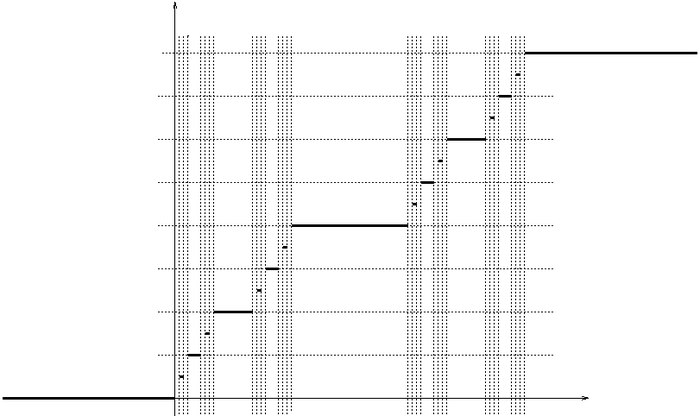
\includegraphics[width=0.8\textwidth]{img/CantorVitaliFunction.png}
\caption{La función de Cantor-Vitali o escalera del diablo.}
\label{fig:CantorVitalFunc}
\end{figure}

Una curiosidad matemática. En la definición de \nlref{def:FuncAbsCont} veíamos que esa era la clase más grande de funciones para las que el teorema fundamental del cálculo con derivada clásica e integral de Lebesgue se cumple. ¿Existe alguna función que sea continua pero no absolutamente continua y que nos sirva de contraejemplo? La respuesta es que sí: es la llamada función de Cantor-Vitali o escalera del diablo.

\begin{defn}[Escalera\IS del diablo] Se construye el conjunto de Cantor y una función que va incrementando en cada ``tercio'' de ese conjunto.
\end{defn}

Sobre el conjunto de Cantor, $f$ es constante, luego $f' = 0$. Sin embargo, la medida del conjunto de Cantor es 1 y por lo tanto la integral no es cero.


\chapter{Ejercicios}
\label{chap:Ejercicios}
% -*- root: ../VariableReal.tex -*-
\section{Hoja 1}

\begin{problem} Sea \meas un espacio de medida.

\ppart Demostrar que $\appl{f}{Ω ⊆ X}{ℝ}$ es medible si y sólo si el conjunto $\set{x ∈ Ω \tq f(x) > r}$ es medible $∀r ∈ ℝ$.
\ppart Demostrar que si la sucesión de funciones $\appl{f_n}{Ω}{ℝ}$ es medible para todo $n$ también lo son las funciones $\sup f_n,\ \inf f_n,\ \limsup f_n$ y $\liminf f_n$.
\ppart Demostrar que si $\appl{f_n}{Ω}{ℝ}$ son medibles y $f_n(x) \convs f(x)$ puntualmente, entonces $f$ es medible.
\solution

\spart

Si $f$ es medible, entonces $∀E ⊆ ℝ$ medible se tiene que $\inv{f}(E)$ es medible, y en particular esto valdrá para los conjuntos de la forma $(r, +∞)$.

Para demostrar la implicación al otro lado, vemos ciertas propiedades de la inversa: sabemos que $μ(\inv{f}(E^c)) = μ(X) - μ(\inv{f}(E))$, que $\inv{f}(E ∩ F) = μ(E)∩μ(F)$ y que $\inv{f}(E∪F) = \inv{f}(E) ∪ \inv{f}(F)$. Así, podemos construir cualquier subconjunto de $ℝ$ a partir de intervalos de la forma $(r, +∞)$, que sabemos que son medibles. Esas operaciones son compatibles con la inversa y entonces podremos descomponerlo todo en conjuntos medibles\footnote{Esto merece algo más de explicación pero bueno.}.

\spart\label{ej:H1:SupremosMedibles} \textit{Nota: esto es una demostración extendida de la \fref{prop:SupremoInfimoMedibles}.}

Para demostrarlo vamos a usar el apartado anterior.

En el caso del supremo, sabemos que $\appl{\sup f_n}{Ω}{ℝ}$ será medible si y sólo si el conjunto \[ \set{x∈Ω \tq \sup_{n∈ℕ} f_n (x) > r } = \bigcup_{n ∈ ℕ} \set{x ∈ Ω \tq f_n(x) > r} \] es medible para todo $r ∈ ℝ$, que lo es porque se puede descomponer como unión de conjuntos medibles. En el caso del ínfimo lo tenemos análogamente pero haciendo la intersección de esos conjuntos: \[ \set{x ∈ Ω \tq \inf_{n∈ℕ} f_n(x) > r} = \bigcap_{n∈ℕ} \set{x∈Ω \tq f_n(x) > r } \]

\spart

Si $f_n \convs f$ puntualmente, eso significa que $\limsup f_n = \liminf f_n = f$, luego por lo que hemos visto en el apartado anterior es efectivamente medible.


\end{problem}

\begin{problem} Probar que si $\appl{f}{ℝ}{ℂ}$ es continua y $f(x) = 0$ en casi todo punto con respecto a la medida de Lebesgue, entonces $f(x) = 0\; ∀x ∈ ℝ$.

\solution

Si $f$ es nula en casi todo punto con respecto a la medida de Lebegue, entonces sólo podemos tener puntos aislados que difieran de 0. Sin embargo, si esos puntos existen no se cumpliría la definición de continuidad.

Más formalmente y usando la definición topológica de continuidad\footnote{No me apetece pensar continuidad en los complejos.} supongamos que existe $a ∈ ℝ$ tal que $c = f(a) ≠ 0$. Dado que $f$ es nula en casi todo punto, $c$ tiene que ser punto aislado y por lo tanto existe un $r ∈ ℝ$ tal que $0 ∉ \bola_r(c) ⊆ ℂ$, es decir, existe un entorno alrededor de $c$ que no contiene a $0$. Sin embargo, si cogemos un entorno $E = (a - ε, a + ε)$, tenemos que $f(E)$ es nulo en casi todo punto, por lo que $f(E) \nsubseteq \bola_r(c)$ y por lo tanto $f$ no puede ser continua. Contradicción, así que $f(x) = 0\; ∀x∈ℝ$.

\end{problem}

\begin{problem} \label{ej:H1:ConvMonotonaSeries} Sea $\set{f_n}$ una sucesión de funciones medibles con $f_n ≥ 0$. Usar el \nref{thm:ConvMonotona} para demostrar que \[ \int_Ω\left(\sum_{n=1}^∞ f_n\right) \dif μ = \sum_{n=1}^∞ \int_Ω f_n \dif μ \]
\solution

Lo cierto es que esto es el \nref{thm:ConvMonotonaSeries}, así que no hay que complicarse mucho la vida. Simplemente hay que definir la sucesión \[ S_N = \sum_{n=1}^N f_n \] que es monótona creciente por ser $f_n ≥ 0$, luego podemos usar el \fref{thm:ConvMonotona}. Lo que tenemos es por lo tanto que  \begin{align*} \int_Ω\left(\sum_{n=1}^∞ f_n\right) \dif μ &= \int_Ω \lim_{N\to \infty} S_N \dif μ \eqexpl{\ref{thm:ConvMonotona}} \lim_{N\to ∞} \int_Ω S_N \dif μ = \\ &= \lim_{N\to ∞} \int_Ω \sum_{n=1}^N f_n \dif μ \eqreasonup{Suma finita} \lim_{N\to ∞} \sum_{n=1}^N \int_Ω f_n \dif μ = \sum_{n=1}^∞ \int_Ω f_n \dif μ \end{align*}

\end{problem}


\nocite{terence10,folland99}

\bibliography{../Apuntes}{}
\printindex
\end{document}
